% Comment this line out if you need a4paper
% \documentclass[letterpaper, 10 pt, conference]{ieeeconf}  


\documentclass[a4paper, 10pt, conference]{ieeeconf}      % Use this line for a4 paper

\IEEEoverridecommandlockouts                              % This command is only needed if 
                                                          % you want to use the \thanks command

\overrideIEEEmargins                                      % Needed to meet printer requirements.

%In case you encounter the following error:
%Error 1010 The PDF file may be corrupt (unable to open PDF file) OR
%Error 1000 An error occurred while parsing a contents stream. Unable to analyze the PDF file.
%This is a known problem with pdfLaTeX conversion filter. The file cannot be opened with acrobat reader
%Please use one of the alternatives below to circumvent this error by uncommenting one or the other
%\pdfobjcompresslevel=0
%\pdfminorversion=4

% See the \addtolength command later in the file to balance the column lengths
% on the last page of the document

% The following packages can be found on http:\\www.ctan.org
%\usepackage{graphics} % for pdf, bitmapped graphics files
%\usepackage{epsfig} % for postscript graphics files
%\usepackage{mathptmx} % assumes new font selection scheme installed
%\usepackage{times} % assumes new font selection scheme installed
%\usepackage{amsmath} % assumes amsmath package installed
%\usepackage{amssymb}  % assumes amsmath package installed
% \addtolength{\topmargin}{50pt}
\title{\LARGE \bf
%Imitating High-Dynamic Human Motion for Full-Sized Humanoid Robot
A Whole-Body Motion Imitation Framework from Human Data for Full-Size Humanoid Robot
% with Motion Retargeting and Model-Based Control
}


\author{Zhenghan Chen$^{1,2^*} $, Haodong Zhang$^{1,2^*}$, Dongqi Wang$^{2,3}$, Jiyu Yu$^{1,2}$, Haocheng Xu$^{1,2}$, \\ Yue Wang$^{1}$, Rong Xiong$^{1,2}$ % <-this % stops a space
\thanks{*The first two authors contributed equally. 1 The State Key Laboratory of Industrial Control and Technology of Zhejiang University. 2 Zhejiang Humanoid Robot Innovation Center. 3 Department of Engineering Mechanics of Zhejiang University. Rong Xiong is the corresponding author. rxiong@zju.edu.cn. This work was supported by the Joint Funds of the National Natural Science Foundation of China (Grant No. U24A20128).}% <-this % stops a space
% \thanks{$^{1}$Zhenghan Chen, Haodong Zhang, Jiyu Yu,Haocheng Xu, Yue Wang, and Rong Xiong are with the State Key Laboratory of Industrial Control and Technology, Zhejiang University, Hangzhou 310027, China. Rong Xiong is the corresponding author
%         {\tt\small rxiong@zju.edu.cn}}%
% \thanks{$^{2}$Dongqi Wang is with the Department of Engineering Mechanics, Zhejiang University, Hangzhou 310027, China.}%
}

\usepackage{array}
\usepackage{amsmath}
\usepackage{amssymb}
% \usepackage{caption}
% \usepackage{booktabs}
\usepackage{hyperref}
\usepackage{bbm}
\usepackage{bm}
\usepackage{stfloats}
\usepackage{subfigure} 
\usepackage{float} % 用于提供额外的浮动参数
\usepackage{multirow}
\usepackage{graphicx}
\usepackage{cleveref}
\usepackage{mathrsfs}
\usepackage{threeparttable}
%\captionsetup{skip=5pt}
\begin{document}

\maketitle
\thispagestyle{empty}
\pagestyle{empty}

%%%%%%%%%%%%%%%%%%%%%%%%%%%%%%%%%%%%%%%%%%%%%%%%%%%%%%%%%%%%%%%%%%%%%%%%%%%%%%%%
\begin{abstract}
Motion imitation is a pivotal and effective approach for humanoid robots to achieve a more diverse range of complex and expressive movements, making their performances more human-like. However, the significant differences in kinematics and dynamics between humanoid robots and humans present a major challenge in accurately imitating motion while maintaining balance. In this paper, we propose a novel whole-body motion imitation framework for a full-size humanoid robot. The proposed method employs contact-aware whole-body motion retargeting to mimic human motion and provide initial values for reference trajectories, and the non-linear centroidal model predictive controller ensures the motion accuracy while maintaining balance and overcoming external disturbances in real time. The assistance of the whole-body controller allows for more precise torque control. Experiments have been conducted to imitate a variety of human motions both in simulation and in a real-world humanoid robot. These experiments demonstrate the capability of performing with accuracy and adaptability, which validates the effectiveness of our approach.
%Traditional methods make a trade off between computational complexity and model accuracy, yet face the dilemma of poor robustness.

\end{abstract}

%%%%%%%%%%%%%%%%%%%%%%%%%%%%%%%%%%%%%%%%%%%%%%%%%%%%%%%%%%%%%%%%%%%%%%%%%%%%%%%%
\section{INTRODUCTION}
% Humanoid robot is a type of robot resembling the human body in shape, capable of performing anthropomorphic motion and interacting with human and environments. And it has become the physical avatar of human beings for executing anthropomorphic operations and locomotive tasks within domestic and industrial settings. Furthermore, their anthropomorphic appearance facilitates interaction and communication with humans, enhancing acceptability, social intimacy, and the intelligibility of their actions \cite{c1,c9}. Anthropomorphic motion, one of the most significant abilities of humanoid robot, is the cornerstone that supports humanoid robot to learn human-specific assignments and improve the performance of anthropomorphic tasks in diverse settings. This enables humanoid robots to imitate human motions, enhancing their capacity to interact with human operators. Unfortunately, it is still a challenge for humanoid robot to perform anthropomorphic motions autonomously. 

Humanoid robot is a type of robot resembling the human body in shape, capable of performing anthropomorphic motion and interacting with human and environments. Anthropomorphic motion, one of the most significant abilities of humanoid robot, is the cornerstone that supports humanoid robot to learn human-specific assignments and improve the performance of anthropomorphic tasks in diverse settings. This enables humanoid robots to imitate human motions, enhancing their capacity to interact with human operators.\cite{c1,c9}. Unfortunately, it is still a challenge for humanoid robot to perform anthropomorphic motions autonomously. 

% demphi, add RL part or not???
Different attempts have been made to endow humanoid robots with anthropomorphic motion capabilities. Traditional methods based on the kinematic and dynamic model analysis focus on how to examine the stability criteria and evaluate the balance while tracking the reference trajectories \cite{c14,c16}, but this type of method lacks the consideration about anthropomorphism of motions. Although the end-to-end reinforcement learning (RL) method combined with adversarial training shows unique advantages of synthesizing and executing graceful and life-like behaviors in simulation\cite{c11,c12}. Another significant method for human-like motion imitation is motion retargeting combined with high-performance controllers, which can achieve the highest similarity in motions. Although combining them organically still faces some challenges, this approach has been widely applied and become the possible solution of anthropomorphic motion imitation \cite{c17}.

% Researchers have targeted different limbs for motion mapping 
% demphi, add neural part 
The first challenge of this combined method is how to deal with the different kinematics and dynamics structures between humans and humanoid robots. Inverse kinematics based on morphing parameter models can improve the accuracy of motions and achieve more natural behaviors, although this may cause the robot to violate its own constraints \cite{c5,c6,c8}. To address this issue, an optimization-based strategy has been introduced, which solves an optimization problem to find the optimal solution while avoiding that the robot approaches its physical constraints limits \cite{c2,c7}. However, these methods required significant time to optimize each motion and may trap in local minimum. Another common strategy is data-driven motion retargeting with the benefits of deep latent variable modeling to overcome these problems \cite{c31}, but it performs inadequately with unfamiliar actions and results in inaccurate movements.

\begin{figure}[t]
      \centering
      \setlength{\abovecaptionskip}{-0.0cm}
      \setlength{\belowcaptionskip}{-0.5cm}
      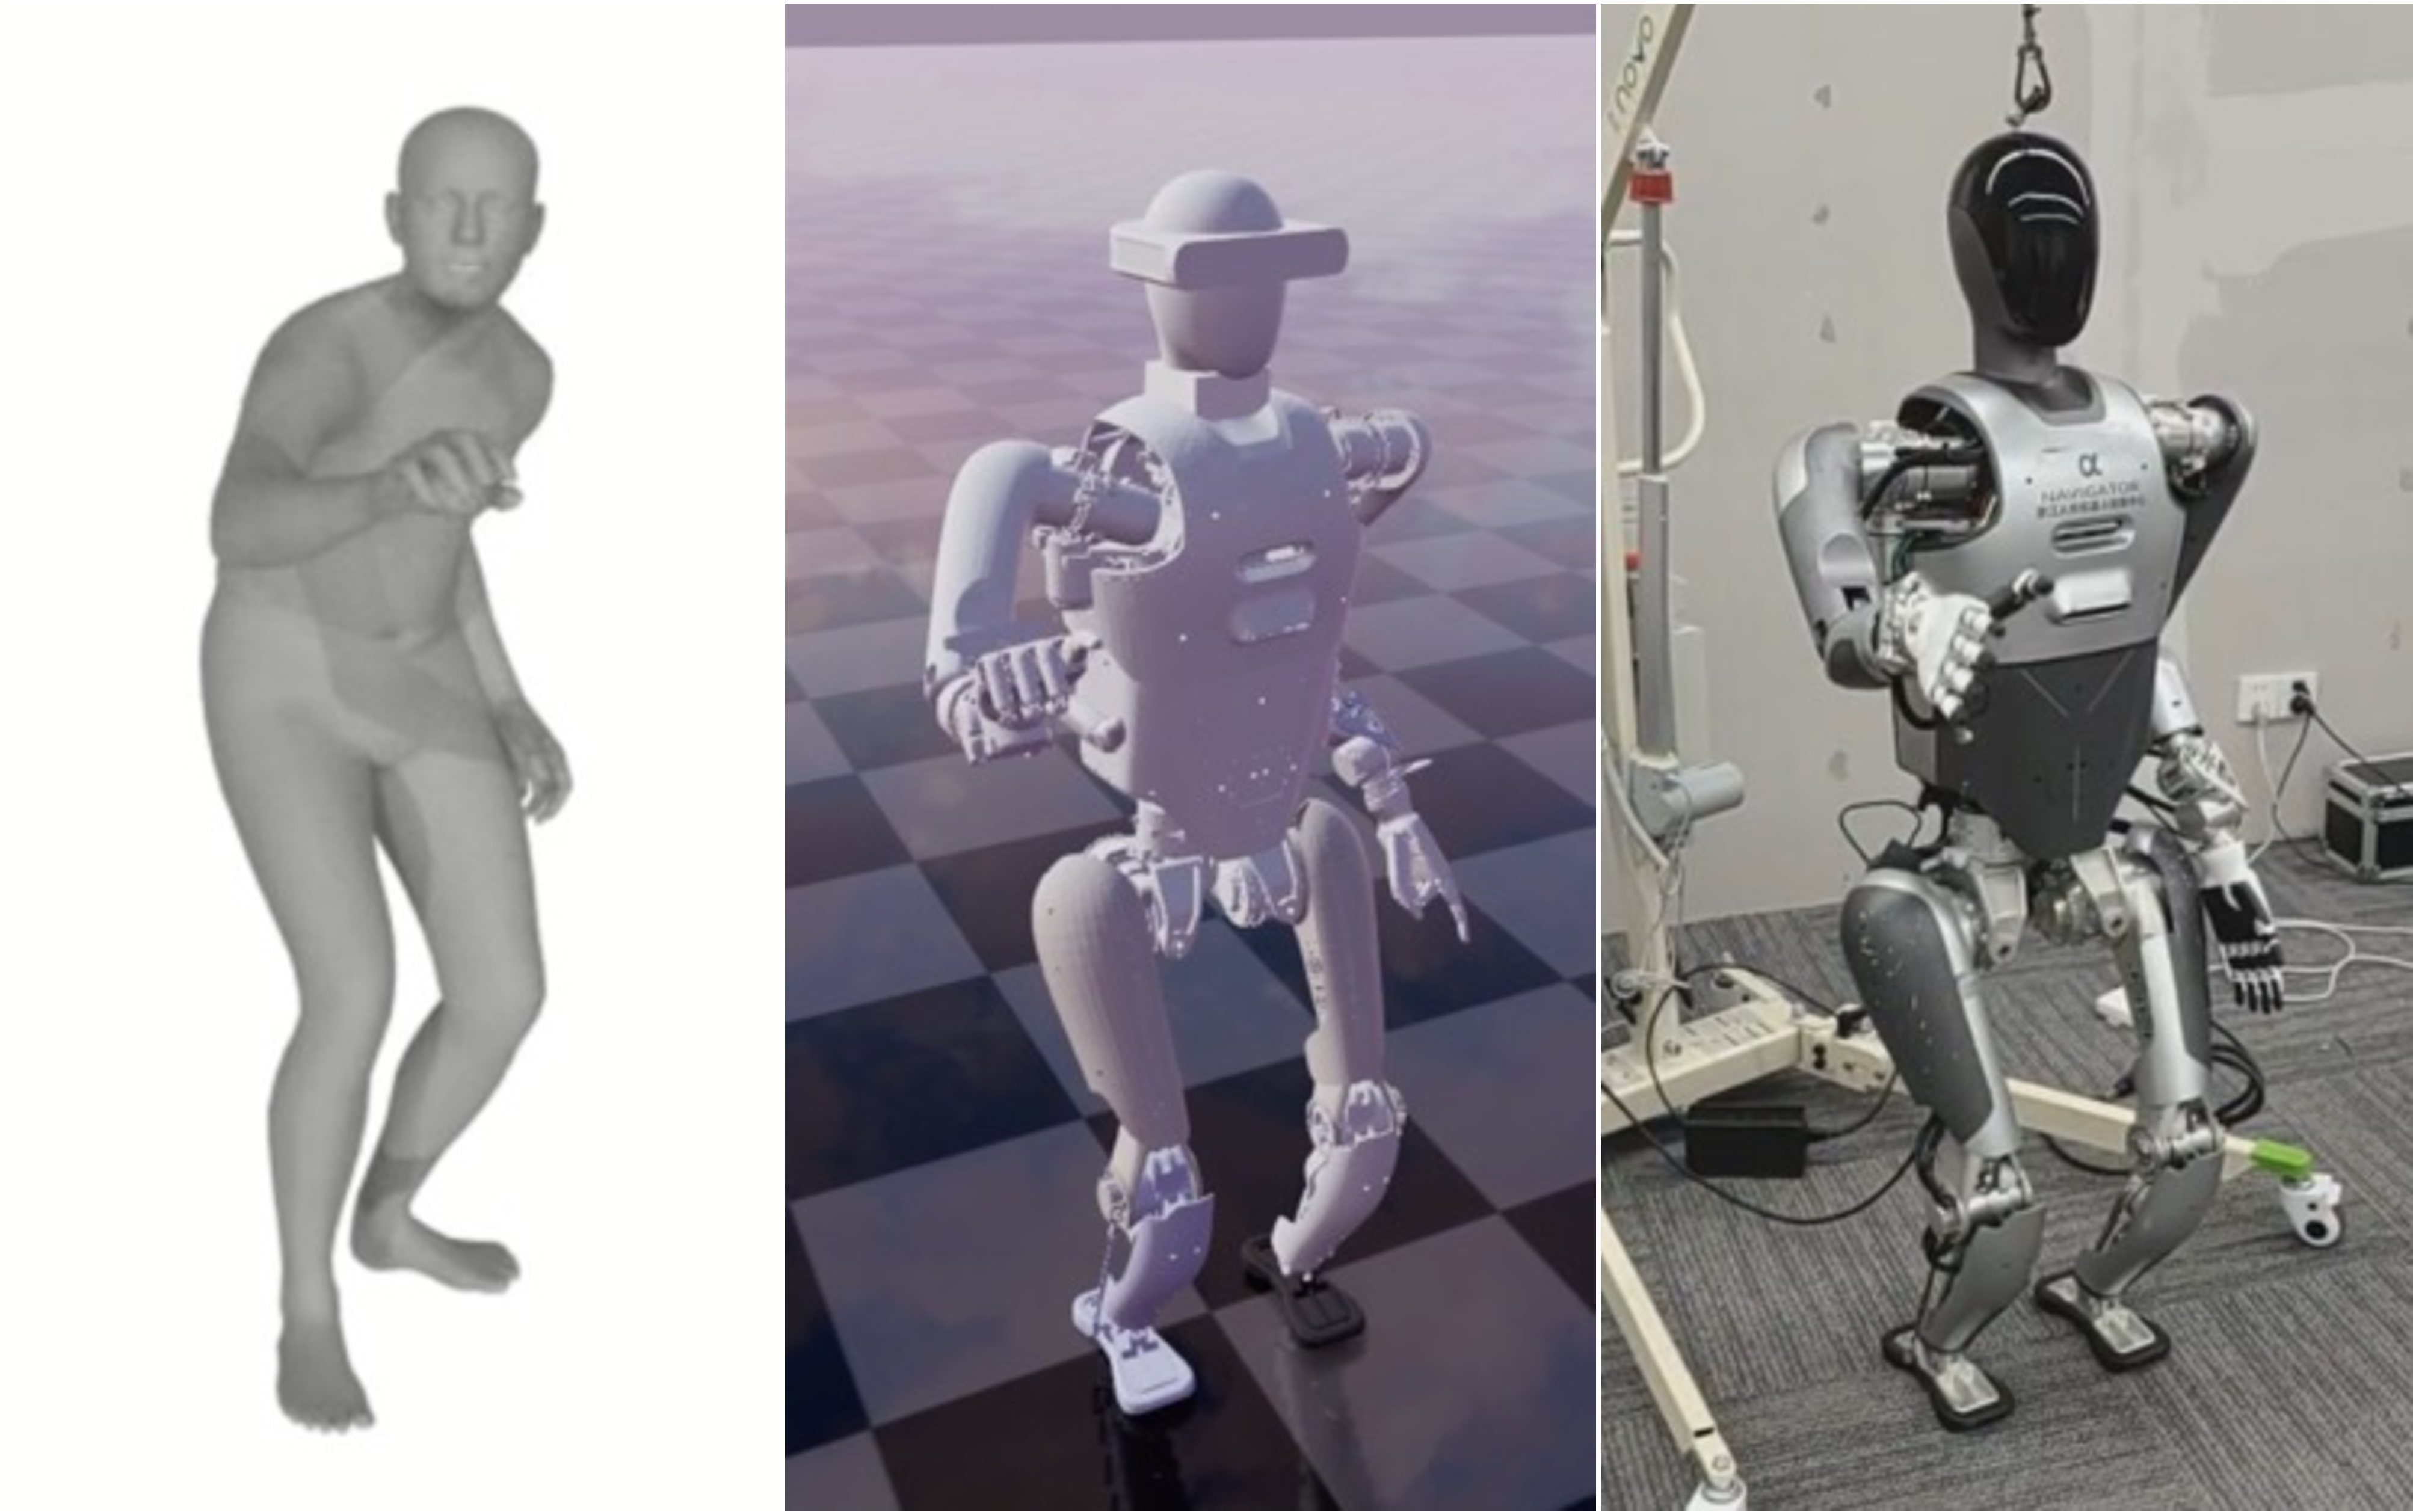
\includegraphics[width=0.4\textwidth]{figures/surface.pdf}
      \caption{The Screenshot of origin human data, and the motion retargeting result of simulation and robot in real world. The motion retargeting considers the physical constraints of robots and remaps the whole-body motion to humanoid robot.}
      \label{fig::surface}
      \vspace{-18pt}
\end{figure}

%  On one hand, offline optimization considers multi rigid body dynamics to achieve the most precise model, sacrificing real-time computation, which can provide a valuable reference trajectory for low-level controllers. However, there is still a long way to go before this strategy can be implemented in real-time to improve the robustness of robots \cite{c13,c16}. 
When performing anthropomorphic motion imitation, the other significant challenge that the combined method faces: ensuring dynamic balance while imitating the human-like motion. Model-based optimization methods have made trade-offs between model complexity and real-time computation. On one hand, offline optimization considers multi rigid body dynamics to achieve the most accurate model, but it sacrifices real-time computation, making it impossible for real-time robot control \cite{c13,c16}. On the other hand, the simplified model method has been used effectively and is computationally efficient for real-time imitation \cite{c3,c14,c15}. However, if the predetermined assumptions are violated, these methods can fail, resulting in unpredictable motion. Model Predictive Control (MPC) instead \cite{c17,c18}, can improve the ability to respond to sudden reactive events and enhance the expressiveness of motions at the same time, which effectively balances the above two algorithms very well.

Therefore, in this paper, we propose a whole-body motion imitation framework for full-size humanoid robots that combines the advantages of motion retargeting and non-linear MPC. The contact-aware whole-body motion retargeting part can provide good initial values for the subsequent controller. The non-linear MPC based on centroidal dynamics can achieve a real-time solution while ensuring the accuracy and stability of the robot's motion imitation, and ensuring that the robot does not violate any nonlinear dynamic constraints. We present results in both simulation and physical platforms, demonstrating the versatility of our proposed method, which has high tracking accuracy while ensuring robot stability. Our contributions are as follows:
\begin{itemize}
\item propose a unified framework consisting of whole-body motion retargeting and model-based control to enable a full-size humanoid robot to imitate human motion data with anthropomorphism and robustness. 
\item introduce whole-body motion retargeting that mimics diverse and expressive human motion while considering foot contact with the environment to provide a high-quality reference trajectory for motion control.
% propose non-linear model predictive control (NMPC) to maintain balance and robustly resist external disturbances while ensuring real-time motion accuracy when performing highly dynamic motions.
\item extend non-linear model predictive control (NMPC)\cite{c37} to whole-body humanoid robot to ensure real-time motion tracking accuracy and maintain balance robustly.
\item our method is tested on a real-world full-size humanoid robot that can perform real-time motion imitation of a wide range of whole-body motions, including upper-body movement, one-legged standing, and other quasi-static motions.
\end{itemize}

\begin{figure*}[ht] % 说明具体的箭头符号
    \vspace{4pt}
    % \setlength{\abovecaptionskip}{-0.3cm}
    % \setlength{\belowcaptionskip}{-0.2cm}
    \centering
    \setlength{\abovecaptionskip}{-0.0cm}
    \setlength{\belowcaptionskip}{-0.2cm}
    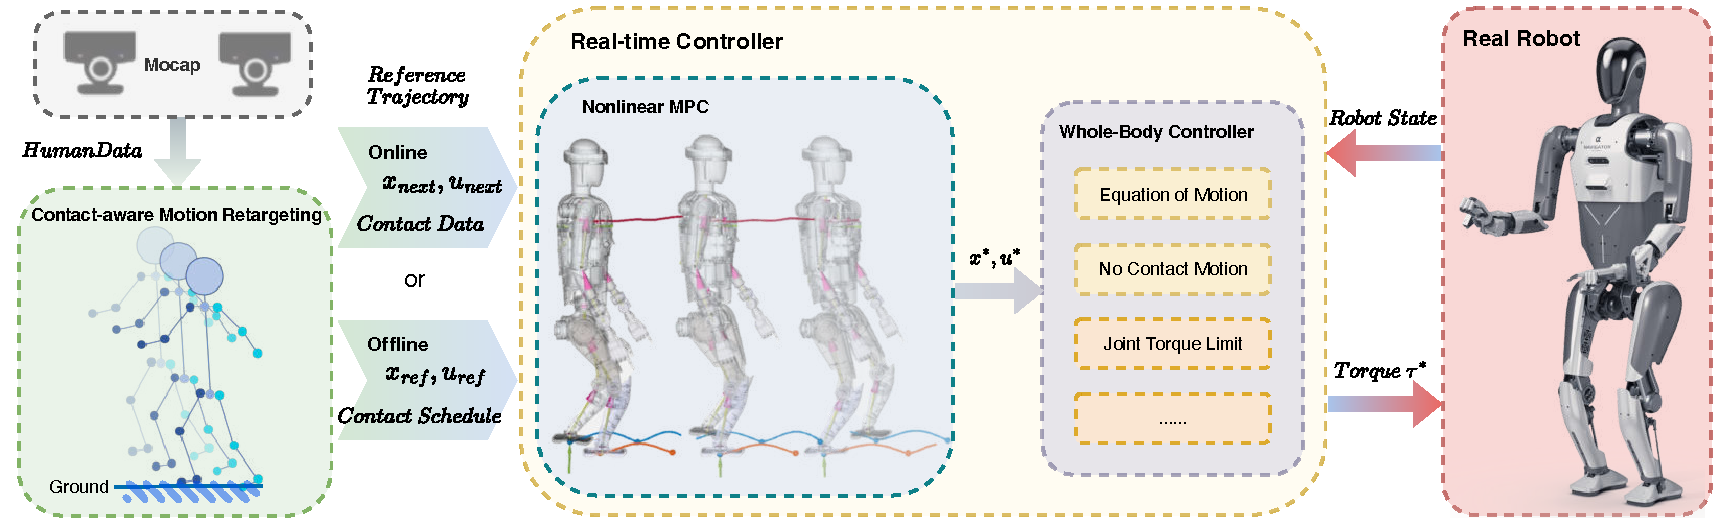
\includegraphics[width=1.0\textwidth]{figures/control-framework.pdf}
    \caption{The overall architecture. We first perform whole-body motion retargeting from human motion data to obtain the online reference trajectory at the next moment($x_{next},u_{next}$) with contact data or the whole offline reference trajectory($x_{ref},u_{ref}$) with the contact schedule. Then, non-linear centroidal model predictive control (NMPC) computes the optimal robot state $x^*$ and the optimal control input $u^*$ while robustly resisting disturbances. Finally, the whole-body controller computes the desired torques $\tau^*$, which are executed by the real full-size humanoid robot.}
    \label{fig::framework}
    \vspace{-17pt}
\end{figure*}

\section{RELATED WORKS}
% Measuring human whole-body motion and kinematically adapting it to robotic motion can improve the robot's anthropomorphic performance.
% add zhang's motion imitation
Motion imitation for humanoid robots using various human data has received considerable attention in recent years due to the human-like structure of robots and their adaptability to various tasks. Miura et al. \cite{c19} presented a method for creating human-like locomotion in humanoid robots by remixing motion capture data, aiming to bridge the gap between human movements and robotic capabilities. Pollard et al. \cite{c20}focused on translating human movements into robotic actions while ensuring stability, efficiency, and naturalness of motion. Zhang et al.\cite{c10} proposed a novel kinematic method that utilizes the advantages of both neural networks and optimization to provide a new perspective for mapping upper-body human motions. Darvish et al. \cite{c21} proposed a method based on inverse kinematics that provided real-time anthropomorphic limb motions for humanoid robot joints. Ishiguro et al. \cite{c22} successfully transferred highly dynamic upper-body and leg motions to the humanoid robot JAXON and demonstrated challenging motions. However, these techniques cannot be used for running and jumping motions and lack robustness. Different from previous techniques, we address the whole-body motion retargeting problem with the foot contact information, yielding the foot contact sequence and timings and providing diverse and anthropomorphic reference trajectory for motion control.

% A common approach is either to keep the center of mass within the support polygon or to keep the net momentum about the center of pressure at zero\cite{c2, c3}.
% while tracking a given trajectory without contact switching, simultaneously achieving balance and tracking. 
% As a result, the achieved stabilization is not robust enough for more challenging motion imitation tasks. 
% With the improvement of computing resources, considering more complex and accurate models of robots has become a trend. 
%  Offline trajectory optimization was introduced by Borno et al. \cite{c25}, who used a LQR-tree formulation to achieve robust physically based retargeting, but still remained in simulation.
% To satisfy equality and inequality constraints in contact forces and to avoid issues such as torque limits, 
Although significant progress has been made in motion retargeting, the other primary challenge in motion imitation is about the controller that ensuring anthropomorphic and stable motion in real time while avoiding falls. Dariush et al. \cite{c14}presents an online task space control retargeting formulation that satisfies balance constraints with a ZMP controller to maintain balance. Yamane et al. \cite{c23} introduced a balance controller based on a simplified robot model and an optimization process to obtain joint torques that enabled a force-controlled robot to maintain balance. However, these methods sacrifice precise models to ensure real-time solving and neglect the re-targeting of torso movements. To satisfy equality and inequality constraints in contact force, Righetti \cite{c24} proposed an inverse dynamic controller that minimizes a combination of linear and quadratic costs. This approach aims to be robust to uncertainties in the dynamic model. Romualdi et al. \cite{c18} proposed an online centroidal MPC formulation for adjusting foot placement, which shows the robustness and potential for more accurate trajectory tracking. As a comparison, our approach integrates real-time non-linear centroidal MPC with contact-aware motion retargeting to guide a humanoid robot imitating anthropomorphic human motion, ensuring accurate and stable motions while maintaining dynamic balance with a better local minimum of the optimization problem.


% \section{MODELING}
% As for a humanoid robot, it is naturally modelled as a system with a free floating-base. We define the generalized coordinates and velocities as : 
% \begin{equation}
%     \bm{q} = \begin{bmatrix}
%         \bm{r}_B \\ \bm{\theta}_B \\ \bm{q}_j 
%     \end{bmatrix} \in \mathbb{R}^{n_q},
%     \bm{\dot{q}} = \begin{bmatrix}  
%         \bm{v}_B \\ \bm{\omega}_B \\ \bm{\dot{q}}_j
%     \end{bmatrix} \in \mathbb{R}^{n_q}
% \end{equation}
% where $n_q = 6+n_j$, $\bm{r}_B \in \mathbb{R}^3$ is the position of the base in the world frame, $\bm{\theta}_B \in \mathbb{R}^3$ is the orientation of the base frame.$\bm{v}_B \in \mathbb{R}^3$ and $\bm{\omega}_B \in \mathbb{R}^3$ are the linear velocity and angular rate of the base in base frame. The limb joint angles and velocities are given by $\bm{q}_j \in \mathbb{R}^{n_j}$ and $\bm{\dot{q}}_j \in \mathbb{R}^{n_j}$, where $n_j = 21$ in this literature. All the subscripts for limbs in contact are contained in the set of $\mathcal{C}$.

% For whole-body dynamics of humanoid robot is given by 

% \begin{equation}
% \label{Eq:dynamics}
%     \bm{M}(\bm{q})\bm{\Ddot{q}}+ \bm{h}(\bm{q}, \bm{\dot{q}}) = \bm{S}^T \bm{\tau} + \bm{J}^T_c(\bm{q})\bm{\lambda}_i
% \end{equation}

% where inertia matrix $\bm{M}(\bm{q}) \in \mathbb{R}^{n_q \times n_q}$ and $\bm{h}(\bm{q}, \bm{\dot{q}}) \in \mathbb{R}^{n_q}$ is the vector of Coriolis, centrifugal and gravity terms. The selection matrix $\bm{S} = [\bm{0}_{n_j \times (n_q-n_j)} \ \mathbb{I}_{n_j \times n_j}]$ selects which DoFs are actuated, resulting to $\bm{S}^T \bm{\tau} = [0 \ \bm{\tau}_j]^T$. The 
% vector of contact wrench $\bm{\lambda} \in \mathbb{R}^{6n_c}$ is mapped to the joint space torques through the contact Jacobian $\bm{J}_c^T \in \mathbb{R}^{6n_c \times n_q}$, which is stacked by the contact Jacobians as $\bm{J}_c^T = [\bm{J}^T_{c_{1}} \ \bm{J}^T_{c_{2}} \ ... \ \bm{J}^T_{c_{n_{c}}} ]^T$, with $n_c$ is the number of limbs in contact.

% Noticed that the contact wrench $\bm{\lambda} = [... \ \bm{f}^T_{c_{1}} \ \bm{\tau}^T_{c_{1}} \ ...]^T$ is the vector of forces $\bm{f}_{c_{i}}$ and torques $\bm{\tau}_{c_{i}}$ acting at the contact points $c_{i}$. We consider the rigid body in contact with a rigid environment through surfaces (e.g., the soles of its feet) rather than points, and assume that the contact surface is described by a rectangle \cite{c36}. This modeling has implications for the friction cone constraint described in Section IV-B.

% It is well known that the top 6 rows of Eq.\ref{Eq:dynamics} are the main interest of underactuated system, and with the proper transformation, in fact, one could equivalently achieved the Newton-Euler equations applied to the robot's center of mass(COM), or so-called centroidal dynamics, which govern the motion of robots \cite{c34,c35}. 

\section{RETARGETING AND CONTROL}

To address the challenging task of whole-body motion imitation from human data for a full-size humanoid robot, we adopt a three-stage pipeline as depicted in \Cref{fig::framework}. The overall framework first generates a high-quality kinematic reference trajectory with foot contact awareness by whole-body motion retargeting, then incorporates dynamic constraints, maintains balance, and resists environmental disturbances by real-time non-linear centroidal MPC, and finally executes the retargeted motion by whole-body controller.

\subsection{Whole-Body Motion Retargeting}
%  with Foot Contact

The objective of whole-body motion retargeting is to mimic the human motion and generate a kinematically feasible reference trajectory for the humanoid robot. The key challenge lies in the morphological differences between human and robot, including link proportions and robot constraints. Given the human motion trajectory, which defined as joint positions $\boldsymbol{P}^{human} \in \mathbb{R}^{T \times n_h \times 3}$, where $n_h$ is the number of human joints and $T$ is the trajectory length, the goal is to obtain the target robot joint angles $\boldsymbol{Q}^{robot} \in \mathbb{R}^{T \times n_j}$, which can be converted to joint positions $\boldsymbol{P}^{robot} \in \mathbb{R}^{T \times n_j \times 3}$ by forward kinematics. Empirically, the robot root state is based on the human pelvis joint and its velocity is scaled according to the corresponding height. The binary foot contact signals are extracted from the original human trajectory by detecting whether the foot height and velocity is close to zero.
% In addition to satisfying joint constraints, our approach also incorporates foot contact constraints, which preserves accurate foot contact and avoids foot sliding.

Here, we extend our previous proposed dual-arm motion retargeting method \cite{c10} to the whole-body task with consideration of foot contact preservation. 
A graph neural network is designed to transform human motion to the robot joint motion. It first encodes the human motion into latent vectors $\boldsymbol{Z}$ using a graph encoder $f_\theta$ and then decodes into target robot motion with a graph decoder $f_\phi$. The graph network models both the human skeleton and robot structure as graphs. The human motion sequence is represented as a spatial temporal graph, where the node features correspond to the joint positions $\boldsymbol{P}^{human}$ and the edge features correspond to joint offsets $\boldsymbol{S}^{human} \in \mathbb{R}^{n_h \times 3}$. Additionally, the robot motion sequence is also represented as a spatial temporal graph, where the node features are transformed from latent vectors to robot joint angles, and the edge features correspond to robot initial offsets and rotations  $\boldsymbol{S}^{robot} \in \mathbb{R}^{n_j \times 6}$.
% To guarantee the satisfaction of joint limit constraints, the output of the network is passed through a $tanh$ non-linear activation function within the ranges from -1 to 1 and then remapped to the lower and upper joint limits. 

\begin{gather}
    \boldsymbol{Z} = f_\theta (\boldsymbol{P}^{human}, \boldsymbol{S}^{human})\\
    \boldsymbol{Q}^{robot} = f_\phi (\boldsymbol{Z}, \boldsymbol{S}^{robot})\\
    \boldsymbol{P}^{robot} = ForwardKinematics(\boldsymbol{Q}^{robot})
\end{gather}

To imitate the human whole-body motion and preserve accurate foot contact, the objective function $L$ is composed of four terms, including the vector similarity loss $L_{vec}$, foot contact loss $L_{foot}$, smoothness loss $L_{smo}$, and self-collision loss $L_{col}$, where $\alpha$, $\beta$, $\gamma$, and $\eta$ are their respective weights.
% Therefore, we formulate the task of whole-body motion retargeting as a constrained optimization problem as Eq.~\ref{Eq:retarget}. The optimization variables are the robot joint angles, which are converted to joint positions by forward kinematics.
% foot contact signals $\boldsymbol{C} \in \mathbbm{R}^{T \times 2}$,
% foot orientation loss $L_{ori}$,  \gamma L_{ori}  $\lambda$

\begin{equation}
\label{Eq:retarget}
    L = \alpha L_{vec} + \beta L_{foot} + \gamma L_{smo} + \eta L_{col}
\end{equation}

The vector similarity loss $L_{vec}$ maintains motion similarity by aligning normalized vectors of key joints between the human and robot. Let $V$ denote the vector set that includes vectors from hips to knees, from knees to ankles, from shoulders to elbows, and from elbows to wrists.

\begin{equation}
    L_{vec} = \sum_t \sum_{\boldsymbol{v}_j \in V} || \boldsymbol{v}_{j,t}^{human} - \boldsymbol{v}_{j,t}^{robot}||
\end{equation}

The foot contact loss $L_{foot}$ preserves the contact with the ground. Let $C$ denote the foot set in contact with the ground. We encourage the contact schedule of the robot to be consistent with the human. Therefore, we minimize the norm of robot foot height and velocity to enforce foot contact.

\begin{equation}
    L_{foot} = \sum_t \sum_{j \in C} || \boldsymbol{p}_{j,t}^{z,robot}|| + ||\boldsymbol{\dot{p}}_{j,t}^{robot}||
\end{equation}

% The foot orientation loss $L_{ori}$ encourages the robot feet to be parallel to the ground to ensure proper contact. Let $y$ and $z$ denote the Y-component and the Z-component respectively of the foot quaternion.

% \begin{equation}
%     L_{ori} = \sum_t || y_t || + || z_t ||
% \end{equation}

The smoothness loss $L_{smo}$ encourages temporal motion consistency by penalizing large deviation of joint positions.

\begin{equation}
    L_{smo} = \sum_t || \boldsymbol{q}_{t} - \boldsymbol{q}_{t-1} ||
\end{equation}

The self-collision loss $L_{col}$ penalizes collision between robot links. The robot links are modelled as capsules. Let $D$ be the link pair set that contains self-collision, and $d_{i,j}$ be the distance between link $i$ and $j$.

\begin{equation}
    L_{col} = \sum_t \sum_{(i,j) \in D}e^{-d_{i,j,t}^2}
\end{equation}

\subsection{Nonlinear Model Predictive Control}
The non-linear centroidal MPC is employed to optimize the state and control input trajectories. However, simultaneously optimizing the motion and the contact schedule is much more difficult than optimizing the motion with a predefined sequence of contacts. Therefore, our nonlinear MPC problem assumes that the contact schedule associated with a given locomotion mode (standing, stepping in place, walking) is given by the user or motion retargeting part. At the same time, a desired base pose and velocity trajectory is provided by the motion retargeting module, which provides an initial guess and helps to simplify the optimization problem.

% new, demphi
We consider to use a direct multi-shooting method for transforming the continue optimization problem into a finite-dimensional nonlinear program(NLP). To satisfy the requirement of real-time iterations, the sequential quadratic programming(SQP) approach based on KKT optimal conditions combined with quadratic approximation strategy \cite{c4} is critical for speeding up. By the way, at each control instance, only one SQP step is performed according to the real-time iteration scheme \cite{c33}.

Now we define the state vector $\bm{x} \in \mathbb{R}^{6+n_q}$ and control input vector $\bm{u} \in \mathbb{R}^{12+n_j}$ during the optimization:
\begin{equation}
\label{eq:state_vector}
    \bm{x} = [\bm{h}_{com}^T \ \bm{r}^T_B \ \bm{\theta}_B^T \ \bm{q}^T_j]^T, \bm{u} = [\bm{f}^T_{c_{1}} \ \bm{\tau}^T_{c_{1}} \ \bm{f}^T_{c_{2}} \ \bm{\tau}^T_{c_{2}} \  \bm{\dot{q}}_j^T]^T
\end{equation}

The continue nonlinear MPC problem formulation is following:
\begin{equation}
\label{eq:MPC}
    \left\{\begin{array}{l} 
    \min\limits_{\bm{u}(\cdot)} \ \bm{\Phi}(\bm{x}(T)) + \int_0^T \bm{l}(\bm{x}(t),\bm{u}(t),t)dt \\
    subject \ to \ \bm{\dot{x}} = f(\bm{x}(t), \bm{u}(t), t) \\
    \bm{g}^1_{eq}(\bm{x}(t), \bm{u}(t), t) = 0 \\
    \bm{g}^2_{eq}(\bm{x}(t),t) = 0 \\
    \bm{h}_{in}(\bm{x}(t),\bm{u}(t),t) \ge 0 \\
    \bm{x}(0) = \bm{x}_0 \\ 
    \end{array}\right.
\end{equation}
where $\bm{x}(t)$ and $\bm{u}(t)$ are the state and control input at time $t$. $\bm{g}^1_{eq}$ represents equality state-input-related constraints, and $\bm{g}^2_{eq}$ represents equality constraints only related to state. $\bm{h}_{in}$ includes state constraints and state-input-related constraints, such as joint position and velocity limits, friction cone constraints, etc. $\bm{x}_0$ is the current measured state of robot.

\textit{1) Cost:}
The cost function $\bm{l}(\bm{x}(t), \bm{u}(t), t)$ is constructed as a least square cost.
\begin{equation}
    \bm{l}_x = ||\bm{x} - \bm{x_{ref}}||_Q, \bm{l}_u = ||\bm{u} - \bm{u_{ref}}||_R
\end{equation}
%$||\cdot||_Q $ means $\frac{1}{2}$.

\textit{2) Equality Constraints:}
For each foot contact point $c_i$, it should obey the following equality constraints:
\begin{equation}
    \label{eq:equality_constraint}
    \left\{\begin{array}{l} 
    \begin{split}
         &\bm{v}_{c_i} = 0  & \text{if} \ c_i \in \mathscr{C}\\
         &\bm{v}_{c_i} \cdot \bm{\hat}{n} = v^*(t) &  \text{if} \ c_i \in \overline{\mathscr{C}}\\ 
         &\bm{f}_{c_i} = 0, \bm{\tau}_{c_i} = 0 & \text{if} \ c_i \in \overline{\mathscr{C}} \\
         % k_p(p_i - p_{ref,i}) = 0 \\
    \end{split}
    \end{array}\right.
\end{equation}
where $v_{c_i}$ is the velocity of the potential contact point. $\mathscr{C}$ represents the point is in contact. The Eq.\ref{eq:equality_constraint} imply the following meanings: the foot of stance leg are not allowed to slip with the ground, the foot of swing leg should track a reference trajectory $v^*(t)$ and the forces will be vanished.

\textit{3) Inequality Constraints:} The inequality includes surface friction cone, joint position and torque limits.
Surface friction cone constraint: 
\begin{equation}
\left\{\begin{array}{l} 
    \mu_{s} f^z_{c_i} - \sqrt{{f^x_{c_i}}^2 + {f^y_{c_i}}^2 + \epsilon^2} \ge 0 \\
    Yf_{c_i}^z - |\tau_{c_i}^x| \ge 0 \\
    Xf_{c_i}^z - |\tau_{c_i}^y| \ge 0 \\
    \tau_{max} \ge \tau_{c_i}^z \ge \tau_{min} \\
    \end{array}\right.
\end{equation}
where $\tau_{min} \triangleq -\mu_s(X+Y)f_{c_i}^z + |Yf_{c_i}^x - \mu_s \tau_{c_i}^x| + |Xf_{c_i}^y - \mu_s \tau_{c_i}^y|$, $\tau_{max} \triangleq + \mu_s(X+Y)f_{c_i}^z - |Yf_{c_i}^x + \mu_s \tau_{c_i}^x| - |Xf_{c_i}^y + \mu_s \tau_{c_i}^y|$ \cite{c36}. $X$ and $Y$ is defined as half the length and width of contact surface.
% which is shown in \Cref{fig::surface_contact}.

% \begin{figure}[h]
%     \centering
%     \vspace{-10pt}
%     \includegraphics[width=0.3\textwidth]{figures/surface contact.png}
%     \caption{The notations used in the surface contact.}
%     \label{fig::surface_contact}
%     \vspace{-10pt}
% \end{figure}

% Joint position and torque limits are described as:
% \begin{equation}
%     \left\{\begin{array}{l} 
%     \bm{q}^{max}_j \ge \bm{q}_j \ge \bm{q}^{min}_j\\
%     \bm{\tau}^{max}_j \ge \bm{\tau}_j \ge -\bm{\tau}^{max}_j\\
%     \end{array}\right.
% \end{equation}

\subsection{Whole-Body Controller}
An optimization-based whole-body controller helps to map the optimized trajectory obtained from the nonlinear MPC to the humanoid robot's joint torque, which considers the full nonlinear rigid body dynamics. While formulating the constrained hierarchical optimization problem, in this work we instead use a single QP to construct the constrained optimization problem, in which the low-priority tasks are embedded in the cost function, and high-priority tasks are treated as constraints. The list of tasks is simuliar to the \cite{c4,c39}.

%\Cref{table_WBC_tasks} displays the list of tasks. The first two blocks of tasks prevent the robot from violating the equality and inequality constraints of torque, force, and joint configuration. And the least squares tasks guide the robot to track the foot motion with a higher weight than the base reference motion, which prevents the robot from taking advantage of leg inertia to track the base motion in underactuated directions \cite{c4}.

% \begin{table}[h]
%     \vspace{5pt}
%     \setlength{\abovecaptionskip}{-0.0cm}
%     \setlength{\belowcaptionskip}{-0.2cm}
%     \caption{WHOLE-BODY CONTROL TASKS}
%     \label{table_WBC_tasks}
%     \centering
%     % \begin{center}
%     \begin{tabular}{c c}
%     \hline
%     \textbf{Type} & \textbf{Task}\\
%     \hline
%     \multicolumn{1}{c}{=} & \begin{tabular}[c]{@{}c@{}}Floating base equations of motion\\ No Motion at the contact points\end{tabular}\\
%     \hline
%     \multicolumn{1}{c}{$\geq$} & \begin{tabular}[c]{@{}c@{}}Torque limits\\ Wrench Friction cone\end{tabular}\\
%     \hline
%     \multicolumn{1}{c}{$Q_i^2||\cdot||^2$} & \begin{tabular}[c]{@{}c@{}} Base Linear and Angular Tracking($Q_i = 1.0$)\\Joint Position Tracking($Q_i = 100.0$)\\ Contact Force Tracking($Q_i = 0.1$)\end{tabular}\\
%     \hline
%     \end{tabular}
%     \vspace{-15pt}
% \end{table}

\section{EXPERIMENTS}

\subsection{Experimental Setup}

We perform experiments on a full-size humanoid robot with 1.5m height, 52kg weight, and 27 degrees of freedom to validate our approach both in simulation and in the real world. And we build the simulation environment in Raisim \cite{c26}. The non-linear MPC runs at an average update rate of 30Hz, with time horizon $T_d=1$s. The MPC problem is solved via OCS2 \cite{c28} and the QP problem in WBC \cite{c39} is solved by qpOASES.

The training dataset for motion retargeting is the large-scale human motion dataset AMASS \cite{c30}. The data is divided into a training set and a test set with a ratio of 8:2. We use Adam optimizer with a learning rate of 1e-4 and a batch size of 16. The training process takes 20 epochs with an NVIDIA GeForce RTX 4090 D GPU and an Intel(R) Core(TM) i9-14900KF CPU. The retargeting network follows the same architecture as \cite{c10}. To adapt to different humanoid robots, the network needs to be retrained.

% \begin{figure*}[ht]
%      \hspace{-10pt}   
%      \vspace{4pt}
%      \setlength{\abovecaptionskip}{0.0cm}
%      \setlength{\belowcaptionskip}{-0.2cm}
     
%     \subfigure[High-level yoga balance with contact sequence]{
%     \begin{minipage}[c]{1.0\linewidth} %自行调整，太大的话会自动换行
%         \centering
%         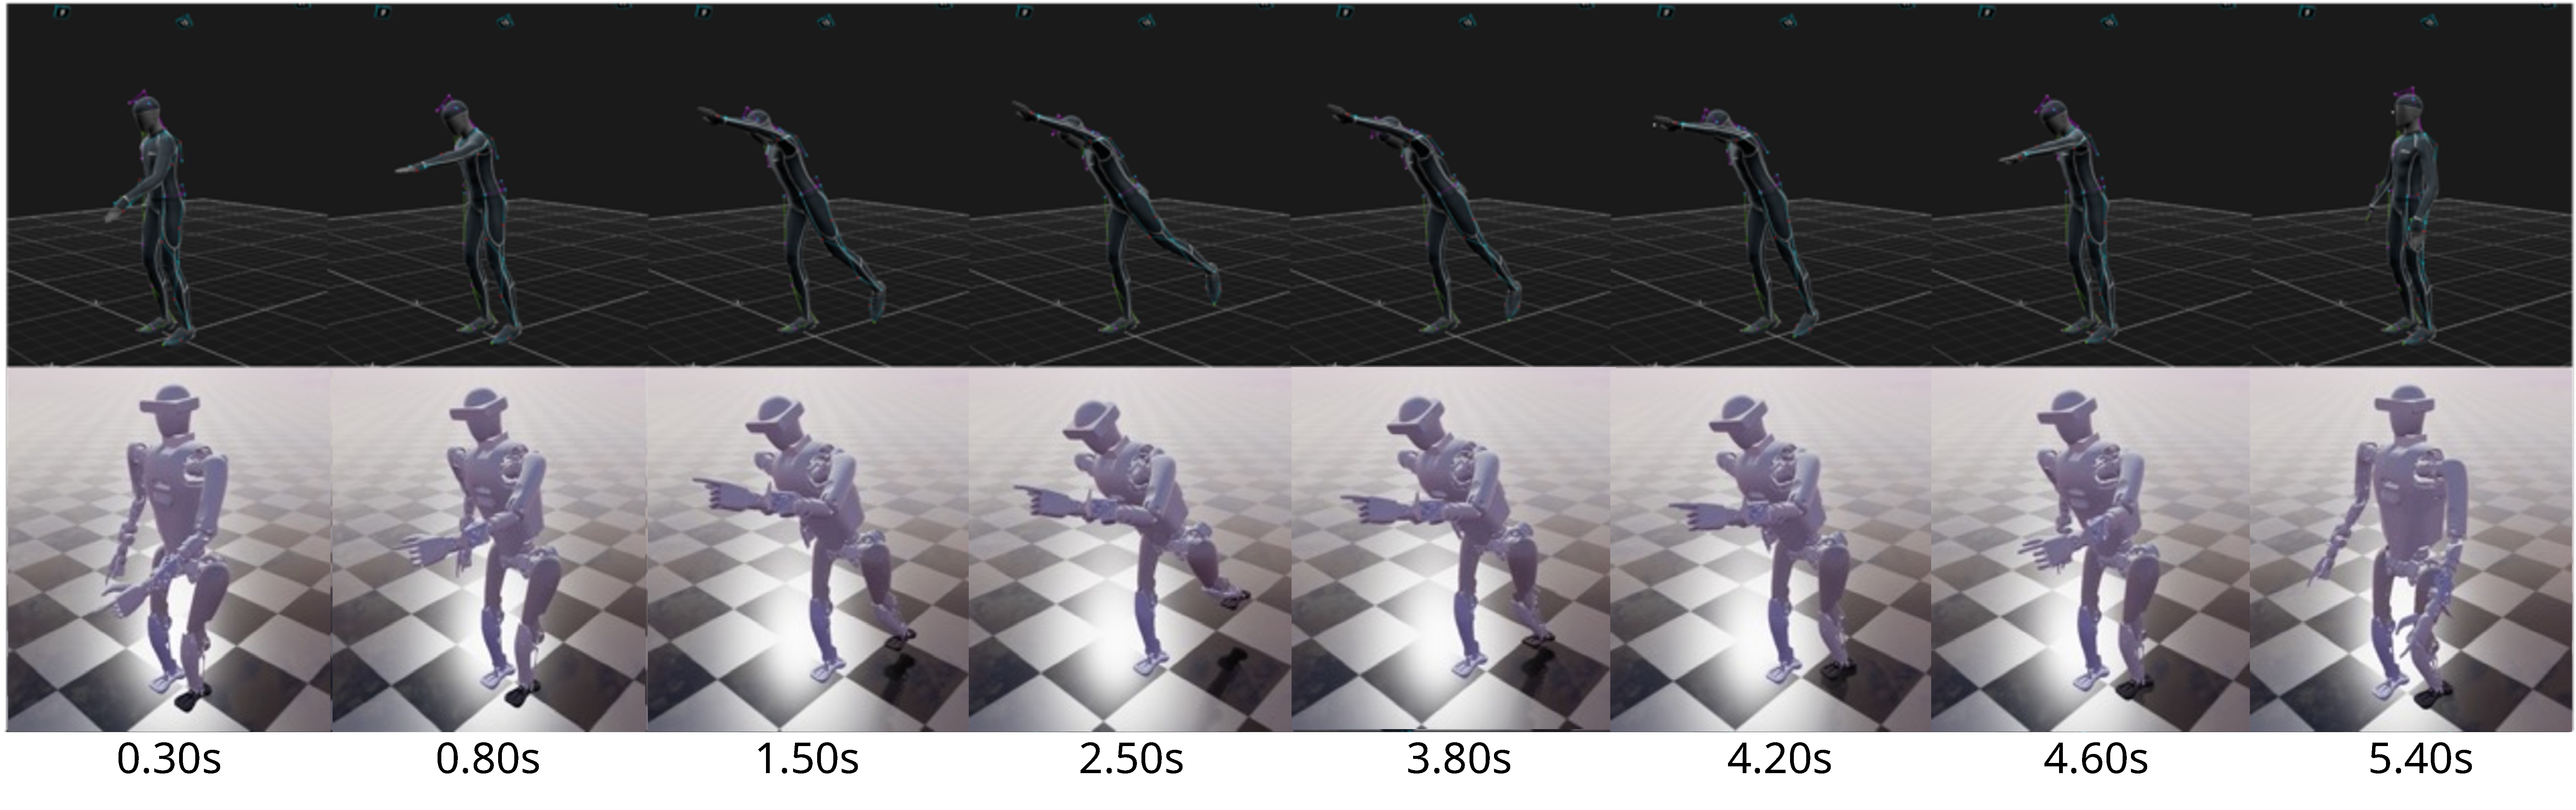
\includegraphics[width=0.98\linewidth]{figures/Motion_yoga.pdf}
%         \vspace{-15pt}  %\vspace需紧跟在后面
%         %width相加大于1时自动换行
%         %自行调整width \vsapce \hspace
%     \end{minipage}
%     }
%     \hspace{-30pt} %调整subfigure的间距
%     \vspace{0pt}
%     \subfigure[High-dynamic stride walking with contact sequence]{
%     \begin{minipage}[c]{1.0\linewidth} %自行调整，太大的话会自动换行
%         \vspace{-5pt}
%         \centering
%         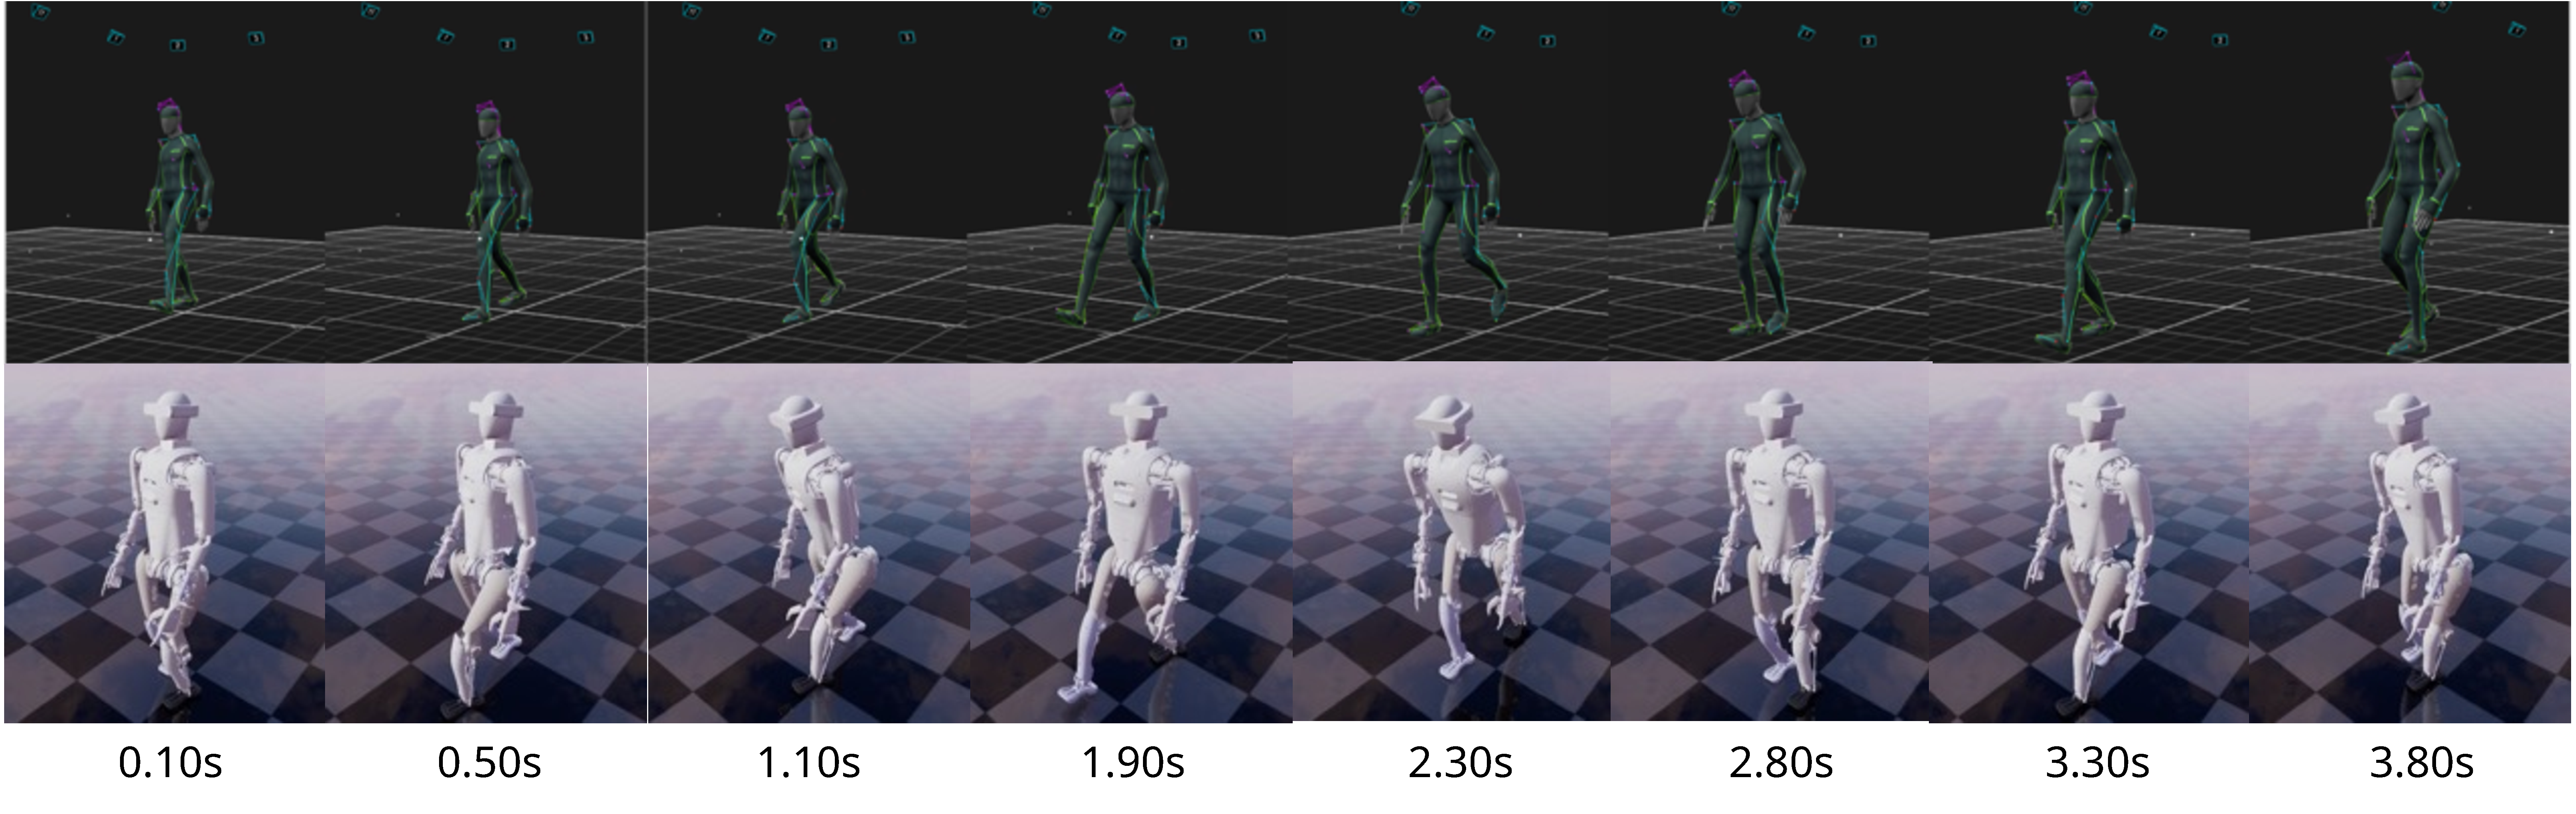
\includegraphics[width=0.98\linewidth]{figures/Motion_stride.pdf}
%         \vspace{-15pt}  %\vspace需紧跟在后面
%         %width相加大于1时自动换行 %自行调整width \vsapce \hspace
%     \end{minipage}
%     }
%     \label{human_motion}
%     \caption{Human motions that are applied to robot by contact-aware motion retargeting.}
%     \vspace{-14pt}
% \end{figure*}

\begin{figure}[ht]
     \hspace{-10pt}   
     \vspace{-10pt}
     \setlength{\abovecaptionskip}{0.0cm}
     \setlength{\belowcaptionskip}{-0.2cm}
     
    \subfigure[High-level yoga balance with contact sequence]{
    \begin{minipage}[c]{0.98\linewidth} %自行调整，太大的话会自动换行
        \centering
        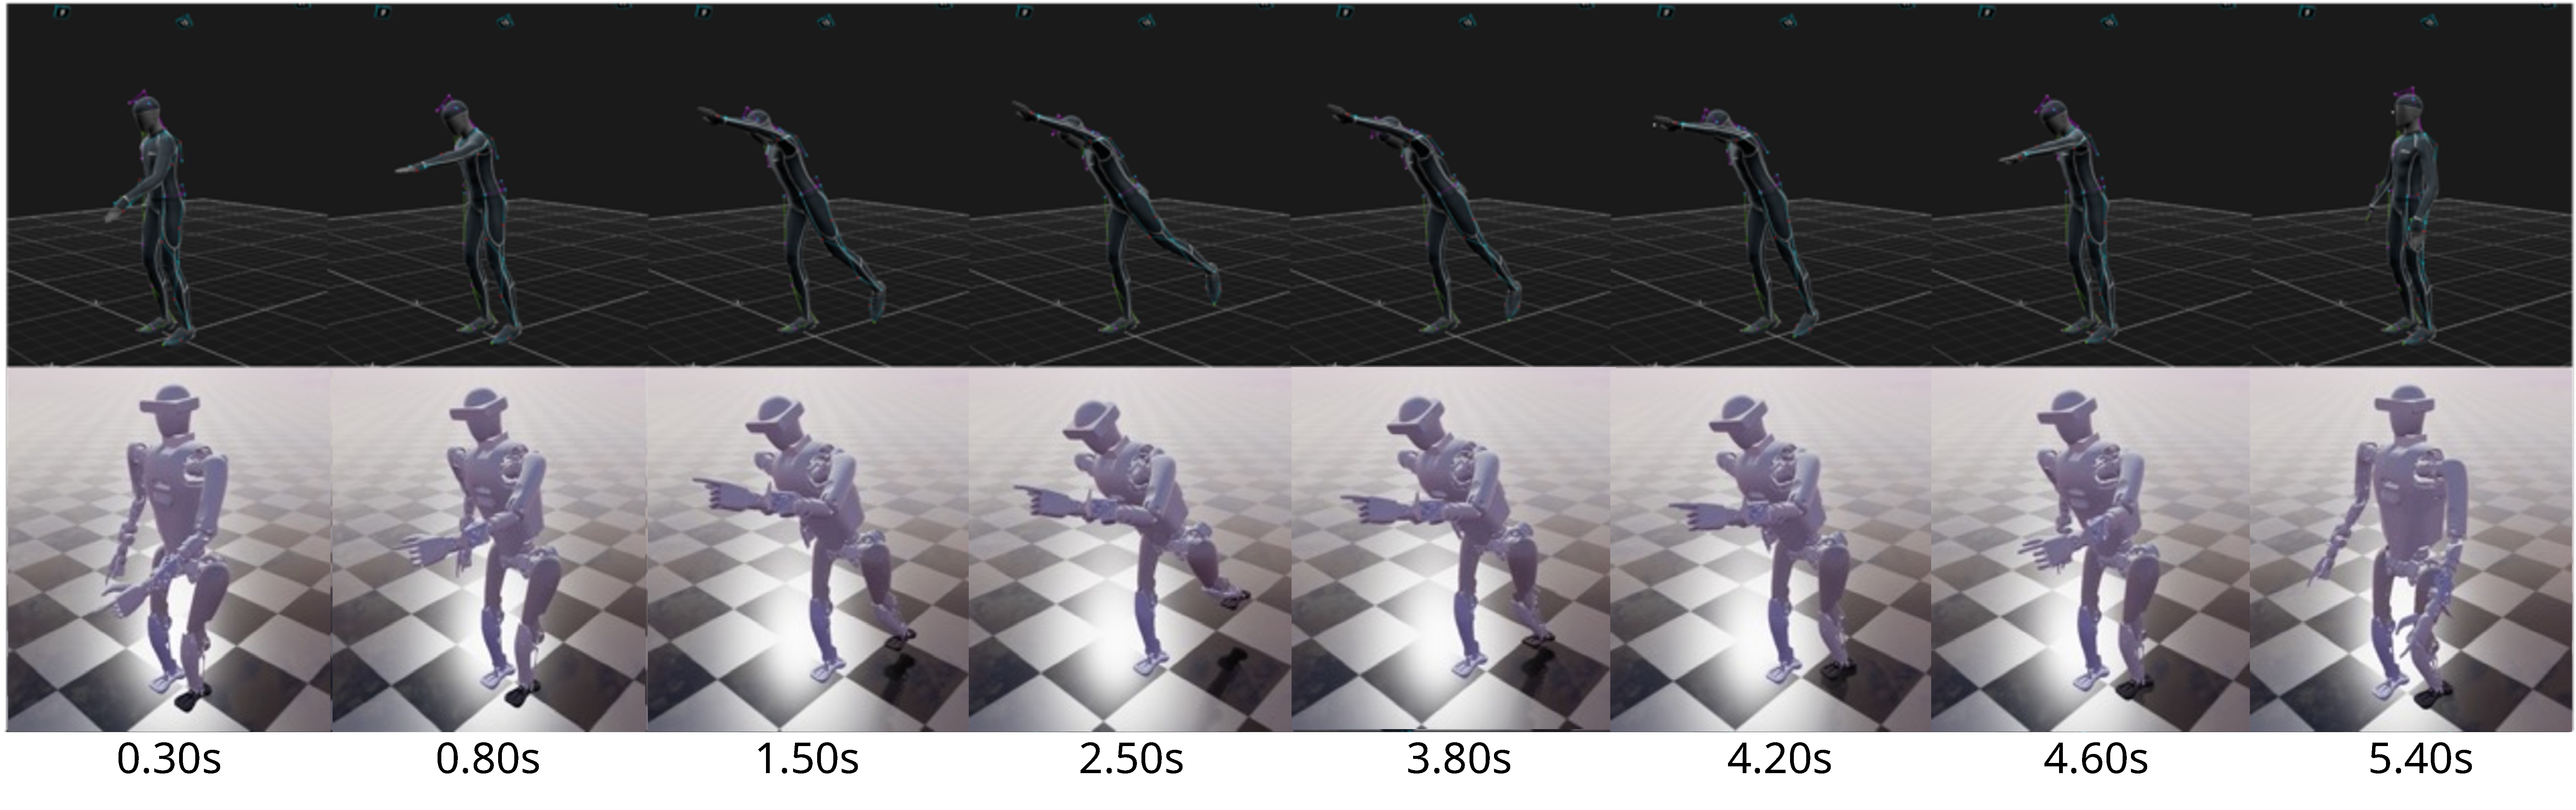
\includegraphics[width=1.0\linewidth]{figures/Motion_yoga.pdf}
        \vspace{-12pt}  %\vspace需紧跟在后面
        %width相加大于1时自动换行
        %自行调整width \vsapce \hspace
    \end{minipage}
    }
    \hspace{-30pt} %调整subfigure的间距
    \vspace{0pt}
    \subfigure[High-dynamic stride walking with contact sequence]{
    \begin{minipage}[c]{0.98\linewidth} %自行调整，太大的话会自动换行
        \vspace{-5pt}
        \centering
        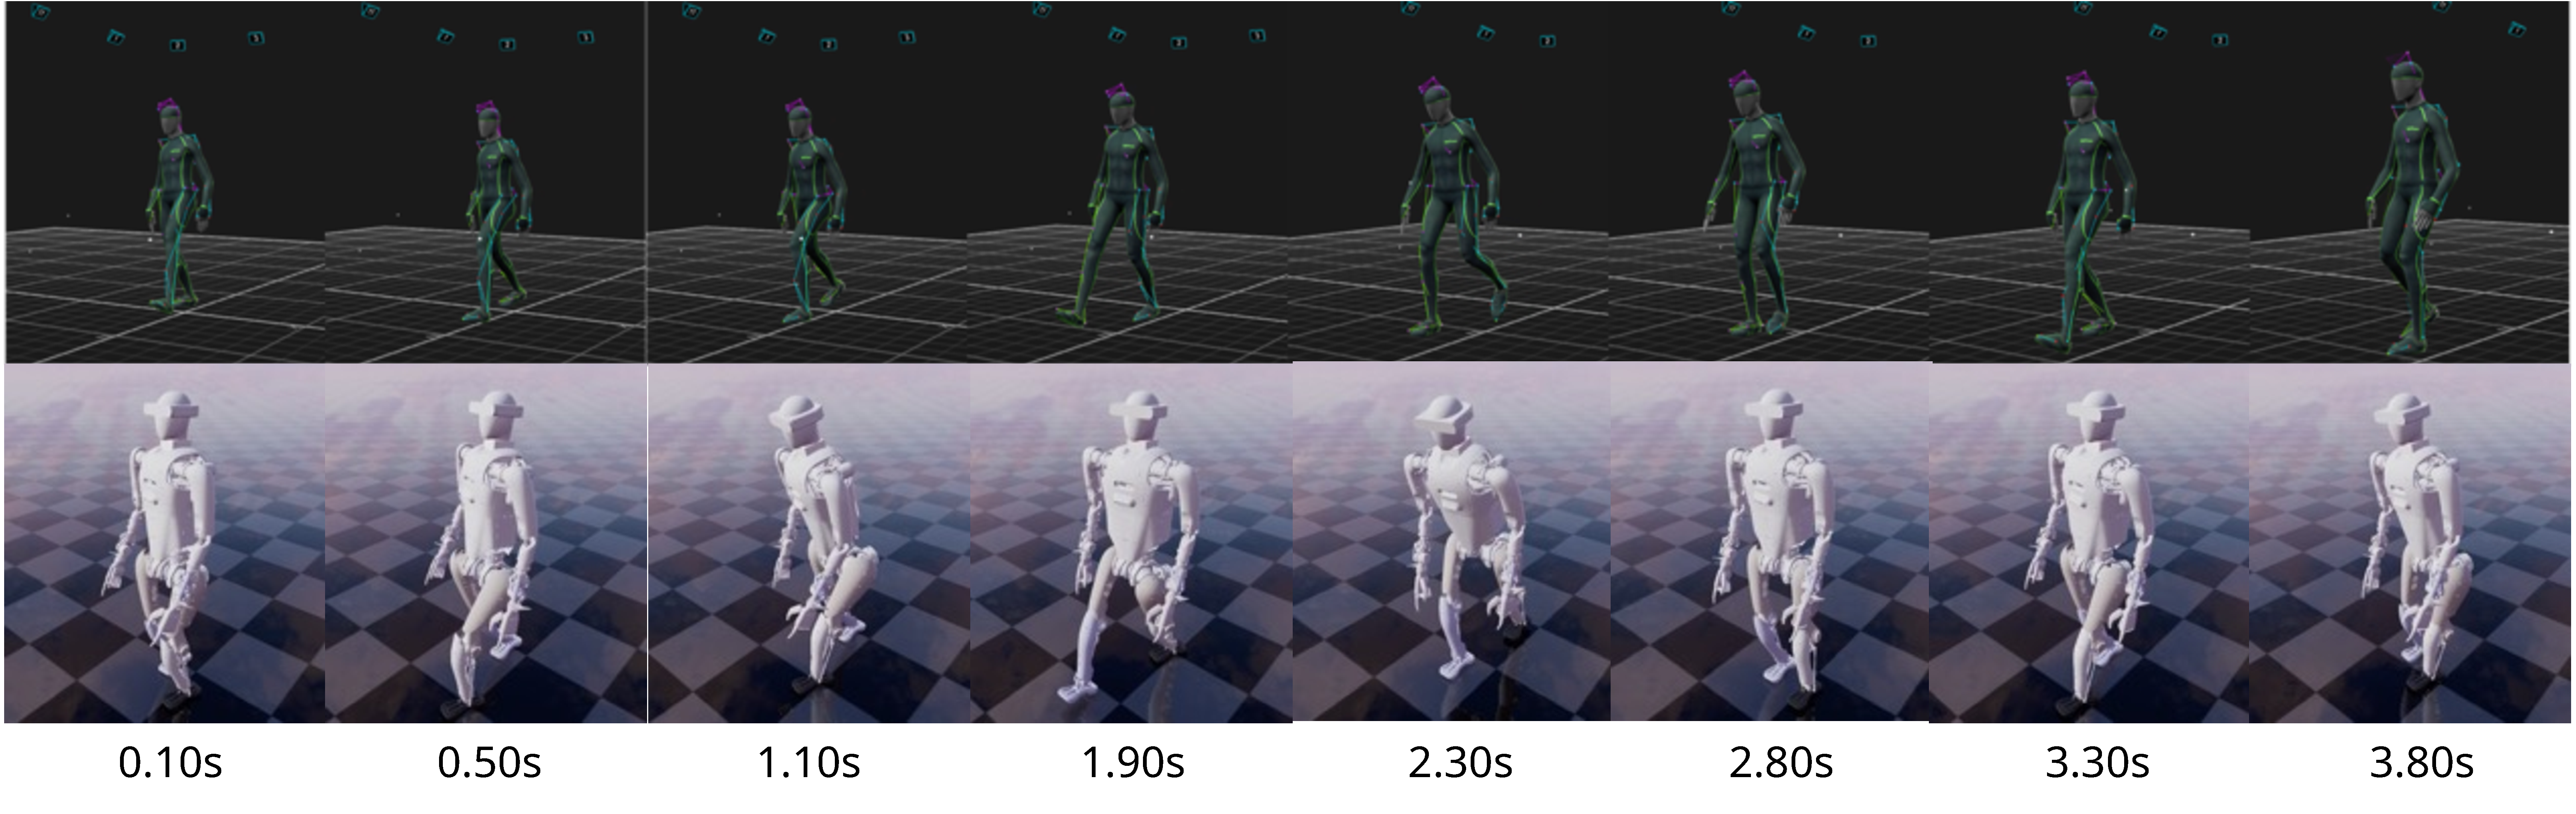
\includegraphics[width=1.0\linewidth]{figures/Motion_stride.pdf}
        \vspace{-12pt}  %\vspace需紧跟在后面
        %width相加大于1时自动换行 %自行调整width \vsapce \hspace
    \end{minipage}
    }
    \caption{Human motions that are applied to robot by contact-aware motion retargeting.}
    \label{fig::human_motion}
    \vspace{-14pt}
\end{figure}

% \subsection{Motion Retargeting Results}
\subsection{Case Study}
% demphi, add real-time details
\noindent\textbf{Offline Motion Retargeting.} We first test our method with pre-recorded human motion data. As shown in the \Cref{fig::human_motion}, our motion retargeting successfully considers the contact sequence between human body and ground contact, and maps it to the robot, successfully performing high-level yoga balance and high-dynamic stride walking motions. 

\noindent\textbf{Online Motion Retargeting.} To achieve real-time online control, the motion retargeting module will generate the reference trajectory for the subsequent moment instead of the whole offline trajectory. The retargeting network generates the robot reference trajectory using a single forward propagation. And linear interpolation will be performed by non-linear MPC module between the current state and the reference trajectory to fill the MPC horizon. As shown in \Cref{fig::online_retargeting}, we can perform real-time online mapping at a frequency of 30Hz, and the average time of each module of the algorithm is shown in \Cref{table_cost_time}.
   \begin{figure}[h]
      \vspace{-5pt}
      \setlength{\abovecaptionskip}{-0.1cm}
      \setlength{\belowcaptionskip}{-0.2cm}
      \centering
      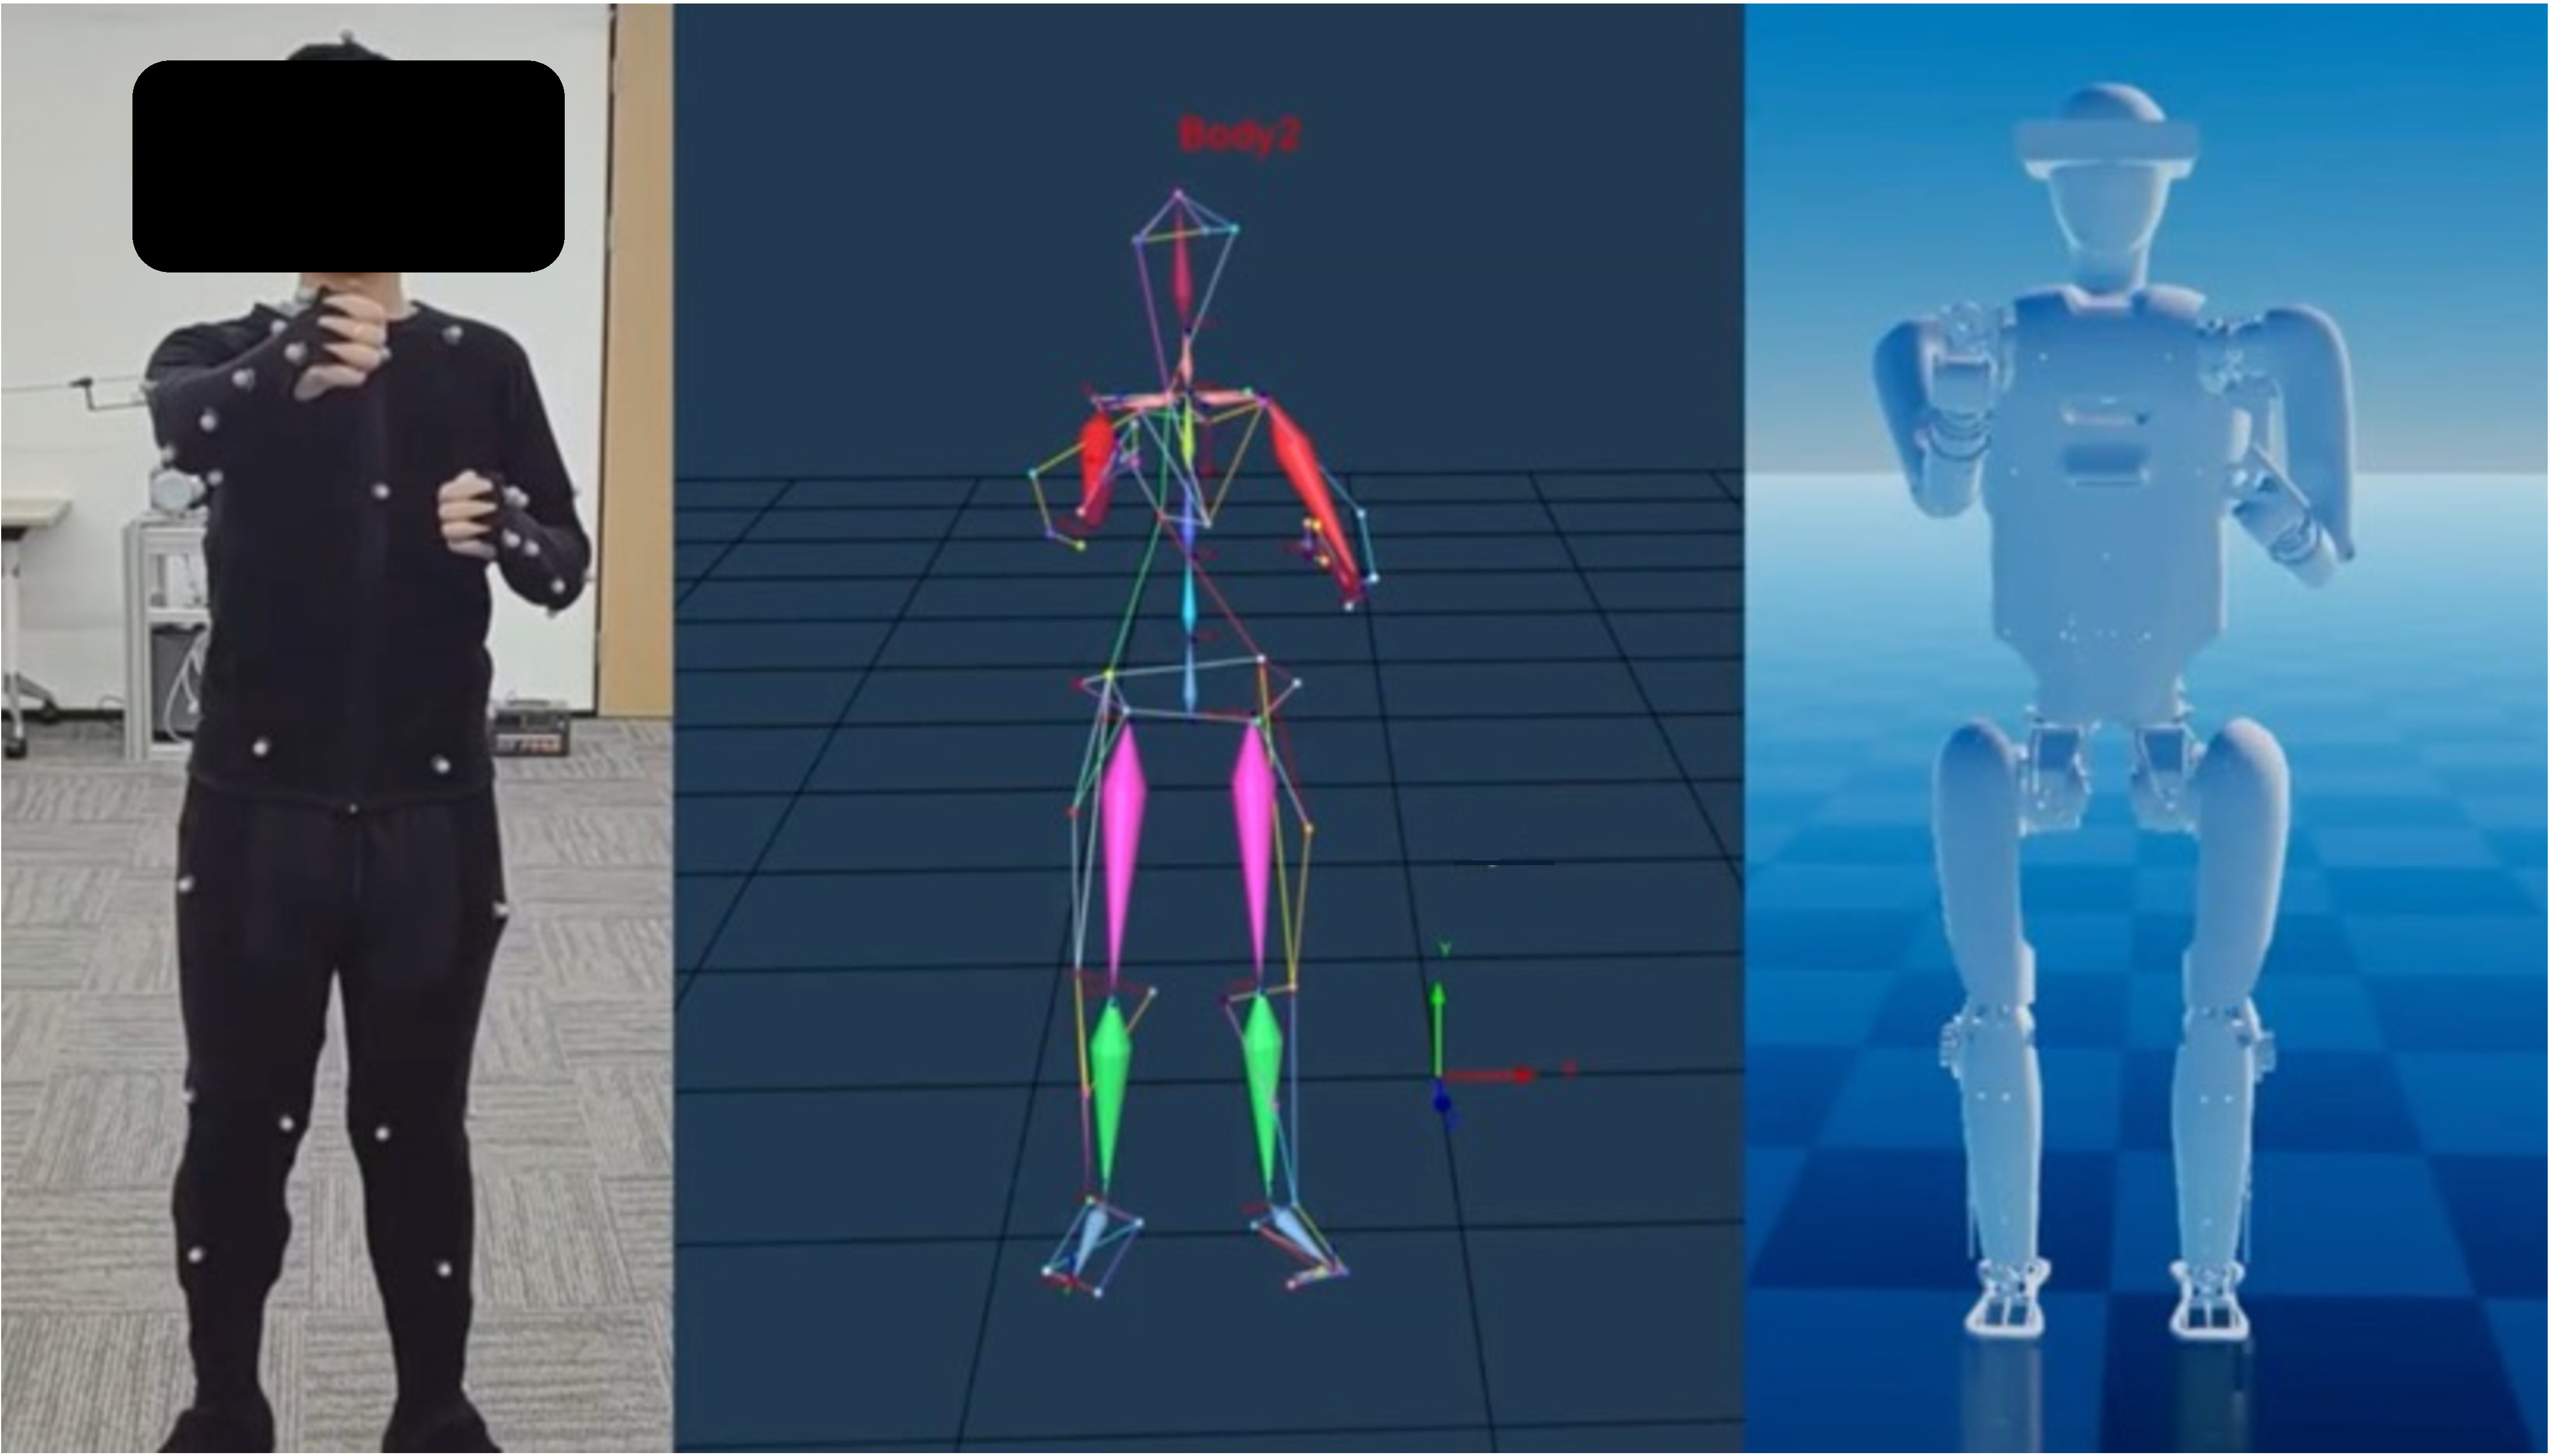
\includegraphics[width=0.25\textwidth]{figures/online_retarget.pdf}
      \caption{The Screenshot of online motion retargeting.}
      \label{fig::online_retargeting}
      \vspace{-15pt}
   \end{figure}

\begin{table}[h]
    \vspace{-5pt}
    \setlength{\abovecaptionskip}{-0.0cm}
    \setlength{\belowcaptionskip}{-0.2cm}
    \caption{COMPUTATION TIME EVALUATION}
    \label{table_cost_time}
    \centering
    \begin{tabular}{ c c c } 
    \hline
    \textbf{Algorithm} & \textbf{Average Time[ms]} & \textbf{Standard Deviation} \\
    \hline
    Motion Retargeting & 11.34 & 3.6907 \\  
    \hline
    Nonlinear MPC & 23.72 & 1.7076 \\  
    \hline
    Whole-Body Control & 0.31 & 0.5644 \\   
    \hline
    \end{tabular}
    \vspace{-8pt}
\end{table}

\noindent\textbf{Push Recovery.}
% demphi, add results analyse
\Cref{fig::stance_walk_push} demonstrates how the humanoid robot overcomes disturbances while keeping stance or walking with proposed MPC controller. The top of pictures show the reaction of MPC controller to the disturbances, and the robot tries to swing its arms for maintaining balance. The bottom plot shows the change of base position $x,y$ and base momentum $h_x,h_y$. Specifically, our non-linear MPC module is able to maintain stable in several steps while robustly resist the external disturbance, which prove the efficiency of our method.

\begin{figure}[ht]
  \vspace{-5pt}
  \setlength{\abovecaptionskip}{-0.2cm}
  \setlength{\belowcaptionskip}{0.2cm}
  \centering
  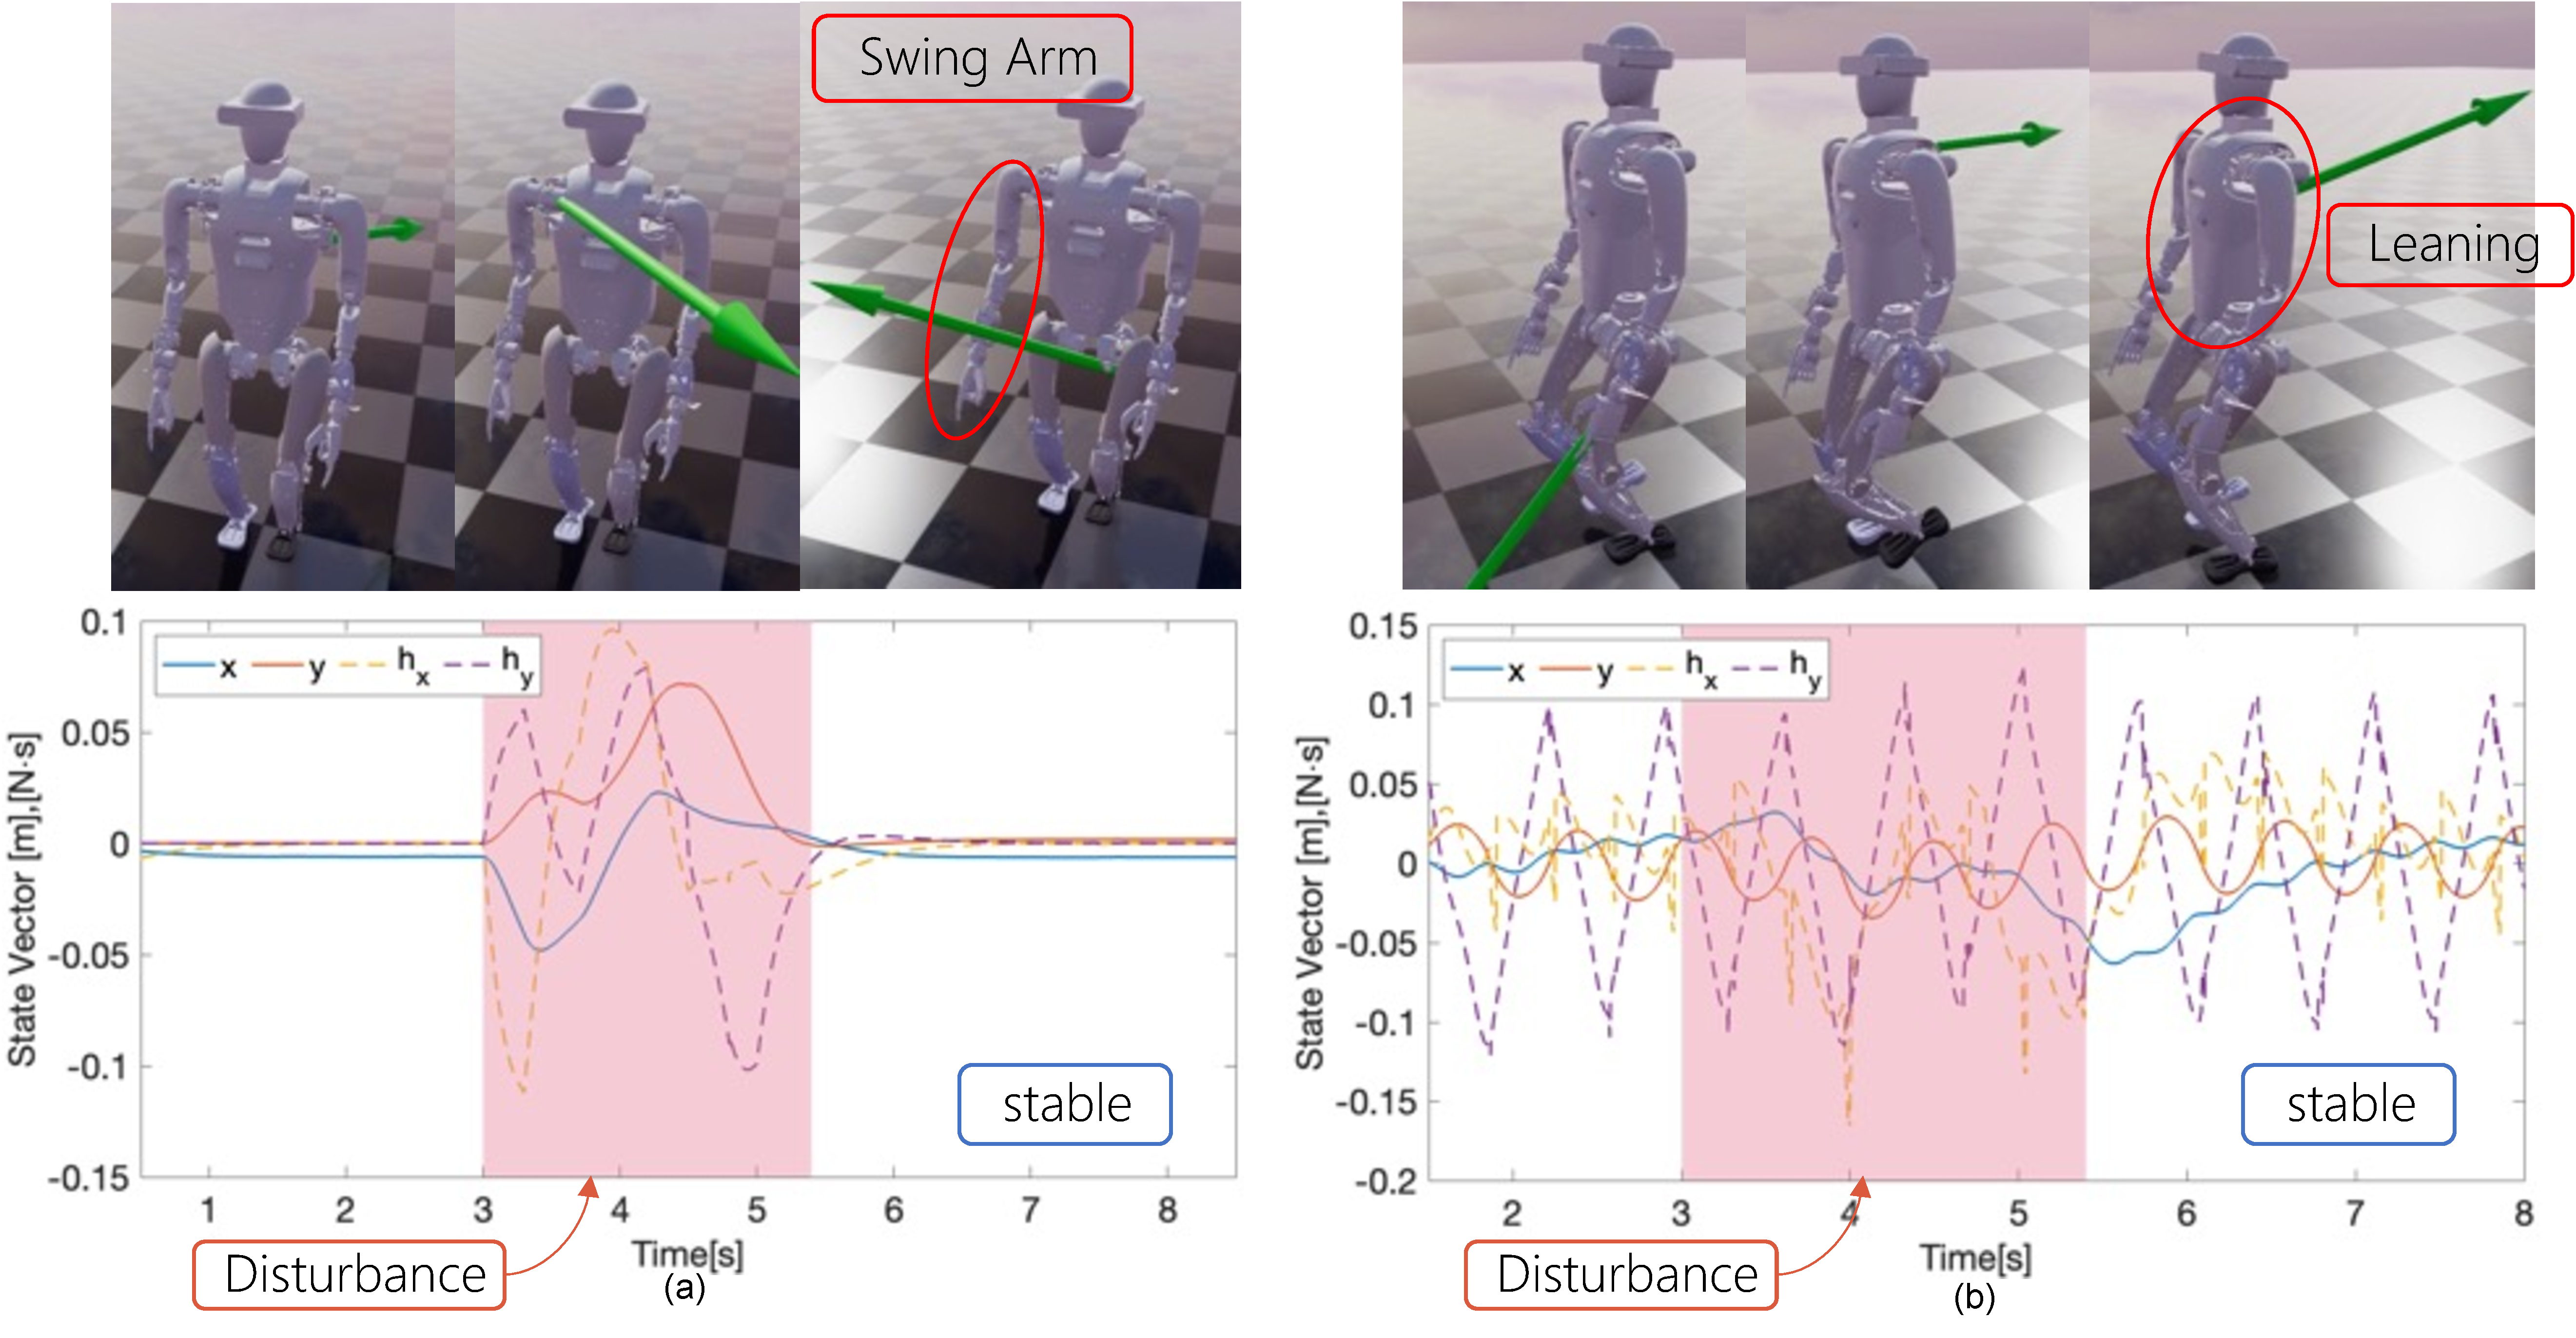
\includegraphics[width=0.47\textwidth]{figures/stance_walk_push.pdf}
  \caption{Simulation results that (a) robot is keeping stance under a disturbance of 140 Ns applied in forward and side direction with the magnitude varies within the range of 70N during the marked time of 2.0s. (b) shows that robot is walking under a disturbance of 150 Ns with the magnitude varies within the range of 50N during the marked time of 2.5s.}
  \label{fig::stance_walk_push}
  \vspace{-10pt}
\end{figure}



\noindent\textbf{Generalization to Another Humanoid Robot.} %\Cref{fig::new_robot} shows our method applied to another humanoid robot, fully demonstrating the generality of our method. 
The details of experiment about the another humanoid robot are shown in the videos \cite{c38}.
   % \begin{figure}[ht]
   %    \vspace{5pt}
   %    \setlength{\abovecaptionskip}{-0.2cm}
   %    \setlength{\belowcaptionskip}{0.2cm}
   %    \centering
   %    \includegraphics[width=0.45\textwidth]{figures/new_robot.pdf}
   %    \caption{Screenshots of motion imitation of another humanoid robot. Pictures(a) and (b) represent different upper-body motions.}
   %    \label{fig::new_robot}
   %    \vspace{-15pt}
   % \end{figure}

% \subsection{Trajectory Tracking}
% \subsection{Quantitative Results}
\subsection{Comparative Study}
To thoroughly evaluate the performance of our approach, we compare the trajectory tracking results in terms of success rate and tracking error with baseline methods. We decide to consider linear MPC approach that uses Single Rigid Body Dynamics(SRBD) as a prediction model \cite{c17} as our baseline. And ablation study of using non-linear MPC module also verifies the effectiveness of our approach, that means the results of motion retargeting will be directly given to WBC \cite{c21}. \Cref{table_compare} shows the success rate of our method, the baseline and the ablation study. Both motions place high demands on the robot's balance and joint tracking capabilities.(The COM and joint tracking accuracy of yoga and stride walking plots are shown in the video.)
% And the \Cref{fig::motion_leg_arm} shows the COM and joint tracking accuracy of yoga and stride walking. 

\begin{table}[h]
    \vspace{-5pt}
    \setlength{\abovecaptionskip}{-0.0cm}
    \setlength{\belowcaptionskip}{-0.2cm}
    \caption{QUANTITATIVE COMPARISON OF DIFFERENT METHODS}
    \centering
    \begin{threeparttable}
    \resizebox{0.47\textwidth}{!}{
        \begin{tabular}{cccccc}
            \hline
            \multirow{2}{*}{\textbf{Motion}} & 
            \multirow{2}{*}{\textbf{Algorithm}} & 
            \multirow{2}{*}{\begin{tabular}[c]{@{}c@{}}\textbf{Success} \\ \textbf{Rate}\end{tabular}} & 
            \multicolumn{3}{c}{\textbf{Average RMSE}} \\ 
            \cline{4-6}
            & & & \multicolumn{1}{c}{\textbf{COM{[}m{]}}} & 
            \multicolumn{1}{c}{\textbf{Leg{[}rad{]}}} & 
            \multicolumn{1}{c}{\textbf{Arm{[}rad{]}}} \\ 
            \hline
            Wave & 
            \begin{tabular}[c]{@{}c@{}c@{}}\textbf{Ours}\\ LMPC+WBC \cite{c17}\\ WBC \cite{c21} \end{tabular} & 
            \begin{tabular}[c]{@{}c@{}c@{}}\textbf{10/10}\\ 10/10\\ 8/10\end{tabular} & 
            \begin{tabular}[c]{@{}c@{}c@{}}\textbf{0.0103}\\ 0.0144\\ 0.0473\end{tabular} & 
            \begin{tabular}[c]{@{}c@{}c@{}}\textbf{0.0535}\\ 0.0643\\ 0.1140\end{tabular} & 
            \begin{tabular}[c]{@{}c@{}c@{}}\textbf{0.0089}\\ 0.0194\\ 0.0882\end{tabular} \\ 
            \hline
            Yoga & 
            \begin{tabular}[c]{@{}c@{}c@{}}\textbf{Ours}\\ LMPC+WBC \cite{c17}\\ WBC \cite{c21} \end{tabular} & 
            \begin{tabular}[c]{@{}c@{}c@{}}\textbf{10/10}\\ 5/10\\ 2/10\end{tabular} & 
            \begin{tabular}[c]{@{}c@{}c@{}}\textbf{0.0170}\\ 0.0400\\ 0.0747\end{tabular} & 
            \begin{tabular}[c]{@{}c@{}c@{}}\textbf{0.1086}\\ 0.1222\\ 0.1893\end{tabular} & 
            \begin{tabular}[c]{@{}c@{}c@{}}\textbf{0.0154}\\ 0.0332\\ 0.1341\end{tabular} \\ 
            \hline
            Stride & 
            \begin{tabular}[c]{@{}c@{}c@{}}\textbf{Ours}\\ LMPC+WBC \cite{c17}\\ WBC \cite{c21} \end{tabular} & 
            \begin{tabular}[c]{@{}c@{}c@{}}\textbf{10/10}\\ 7/10\\ -\end{tabular} & 
            \begin{tabular}[c]{@{}c@{}c@{}}\textbf{0.0472}\\ 0.0598\\ -\end{tabular} & 
            \begin{tabular}[c]{@{}c@{}c@{}}\textbf{0.1299}\\ 0.1901\\ -\end{tabular} & 
            \begin{tabular}[c]{@{}c@{}c@{}}\textbf{0.0359}\\ 0.0405\\ -\end{tabular} \\ 
            \hline
        \end{tabular}
    }
    \begin{tablenotes}
      % \footnotesize   % 添加命令
        \item[*] LMPC+WBC \cite{c17} denotes that Linear MPC combined with WBC.
        \item[-] means it failed to complete motion %自己改注释 和表格对应
    \end{tablenotes}
    \label{table_compare}
    \end{threeparttable}
    \vspace{-10pt}
\end{table}

% add, demphi, about baseline and ablation study
Notice that compared to linear MPC method, our proposed approach considers a more precise dynamic model and reduces the violation of nonlinear constraints, while slightly improve the tracking accuracy and the success rate of high dynamic motions. Considering ablation study, the non-linear MPC module synthesizes the motion stability within the prediction horizon and enhance the ability to respond to sudden reactive events, which improves both accuracy and robustness.

Since the leg joints are more crucial for maintaining the balance of the humanoid robot, and given the limited dynamic model information in the retargeting process, MPC will control the leg joints to adopt strategies that slightly deviate from the retargeting results in order to best satisfy the robot's centroidal dynamics equation without violating nonlinear constraints. The tracking performance of the arm joints exceeds that of the leg joints. 

   % \begin{figure*}[ht]
   %    \vspace{4pt}
   %    \setlength{\abovecaptionskip}{-0.2cm}
   %    \setlength{\belowcaptionskip}{0.2cm}
   %    \centering
   %    \includegraphics[width=1.0\textwidth]{figures/motion_leg_arm.pdf}
   %    \caption{From left to right, the plots show the tracking status of the COM, leg joint, and arm joint. The Average RMSE is showed in \Cref{table_compare}. Obviously, the tracking performance of the arm joints outperforms that of the leg joints. (a) the results of yoga, (b) the results of stride.}
   %    \label{fig::motion_leg_arm}
   %    % \vspace{-5pt}
   % \end{figure*}

\subsection{Real World Experiment}
Our approach was testified in the humanoid robot hardware together with the state estimator. We had verified the upper-body motion while robot in stance state keeping balance, and also completed the task of standing on one leg. \Cref{fig::real_robot} shows the screenshots of the real world experiments, and for each motion we tested five times without failure. The robot employing our strategy is also capable of performing simple walking tasks, shown in the videos \cite{c38}. 

\begin{figure}[ht]
      \vspace{-10pt}
      \setlength{\abovecaptionskip}{-0.3cm}
      \setlength{\belowcaptionskip}{-0.2cm}
      \centering
      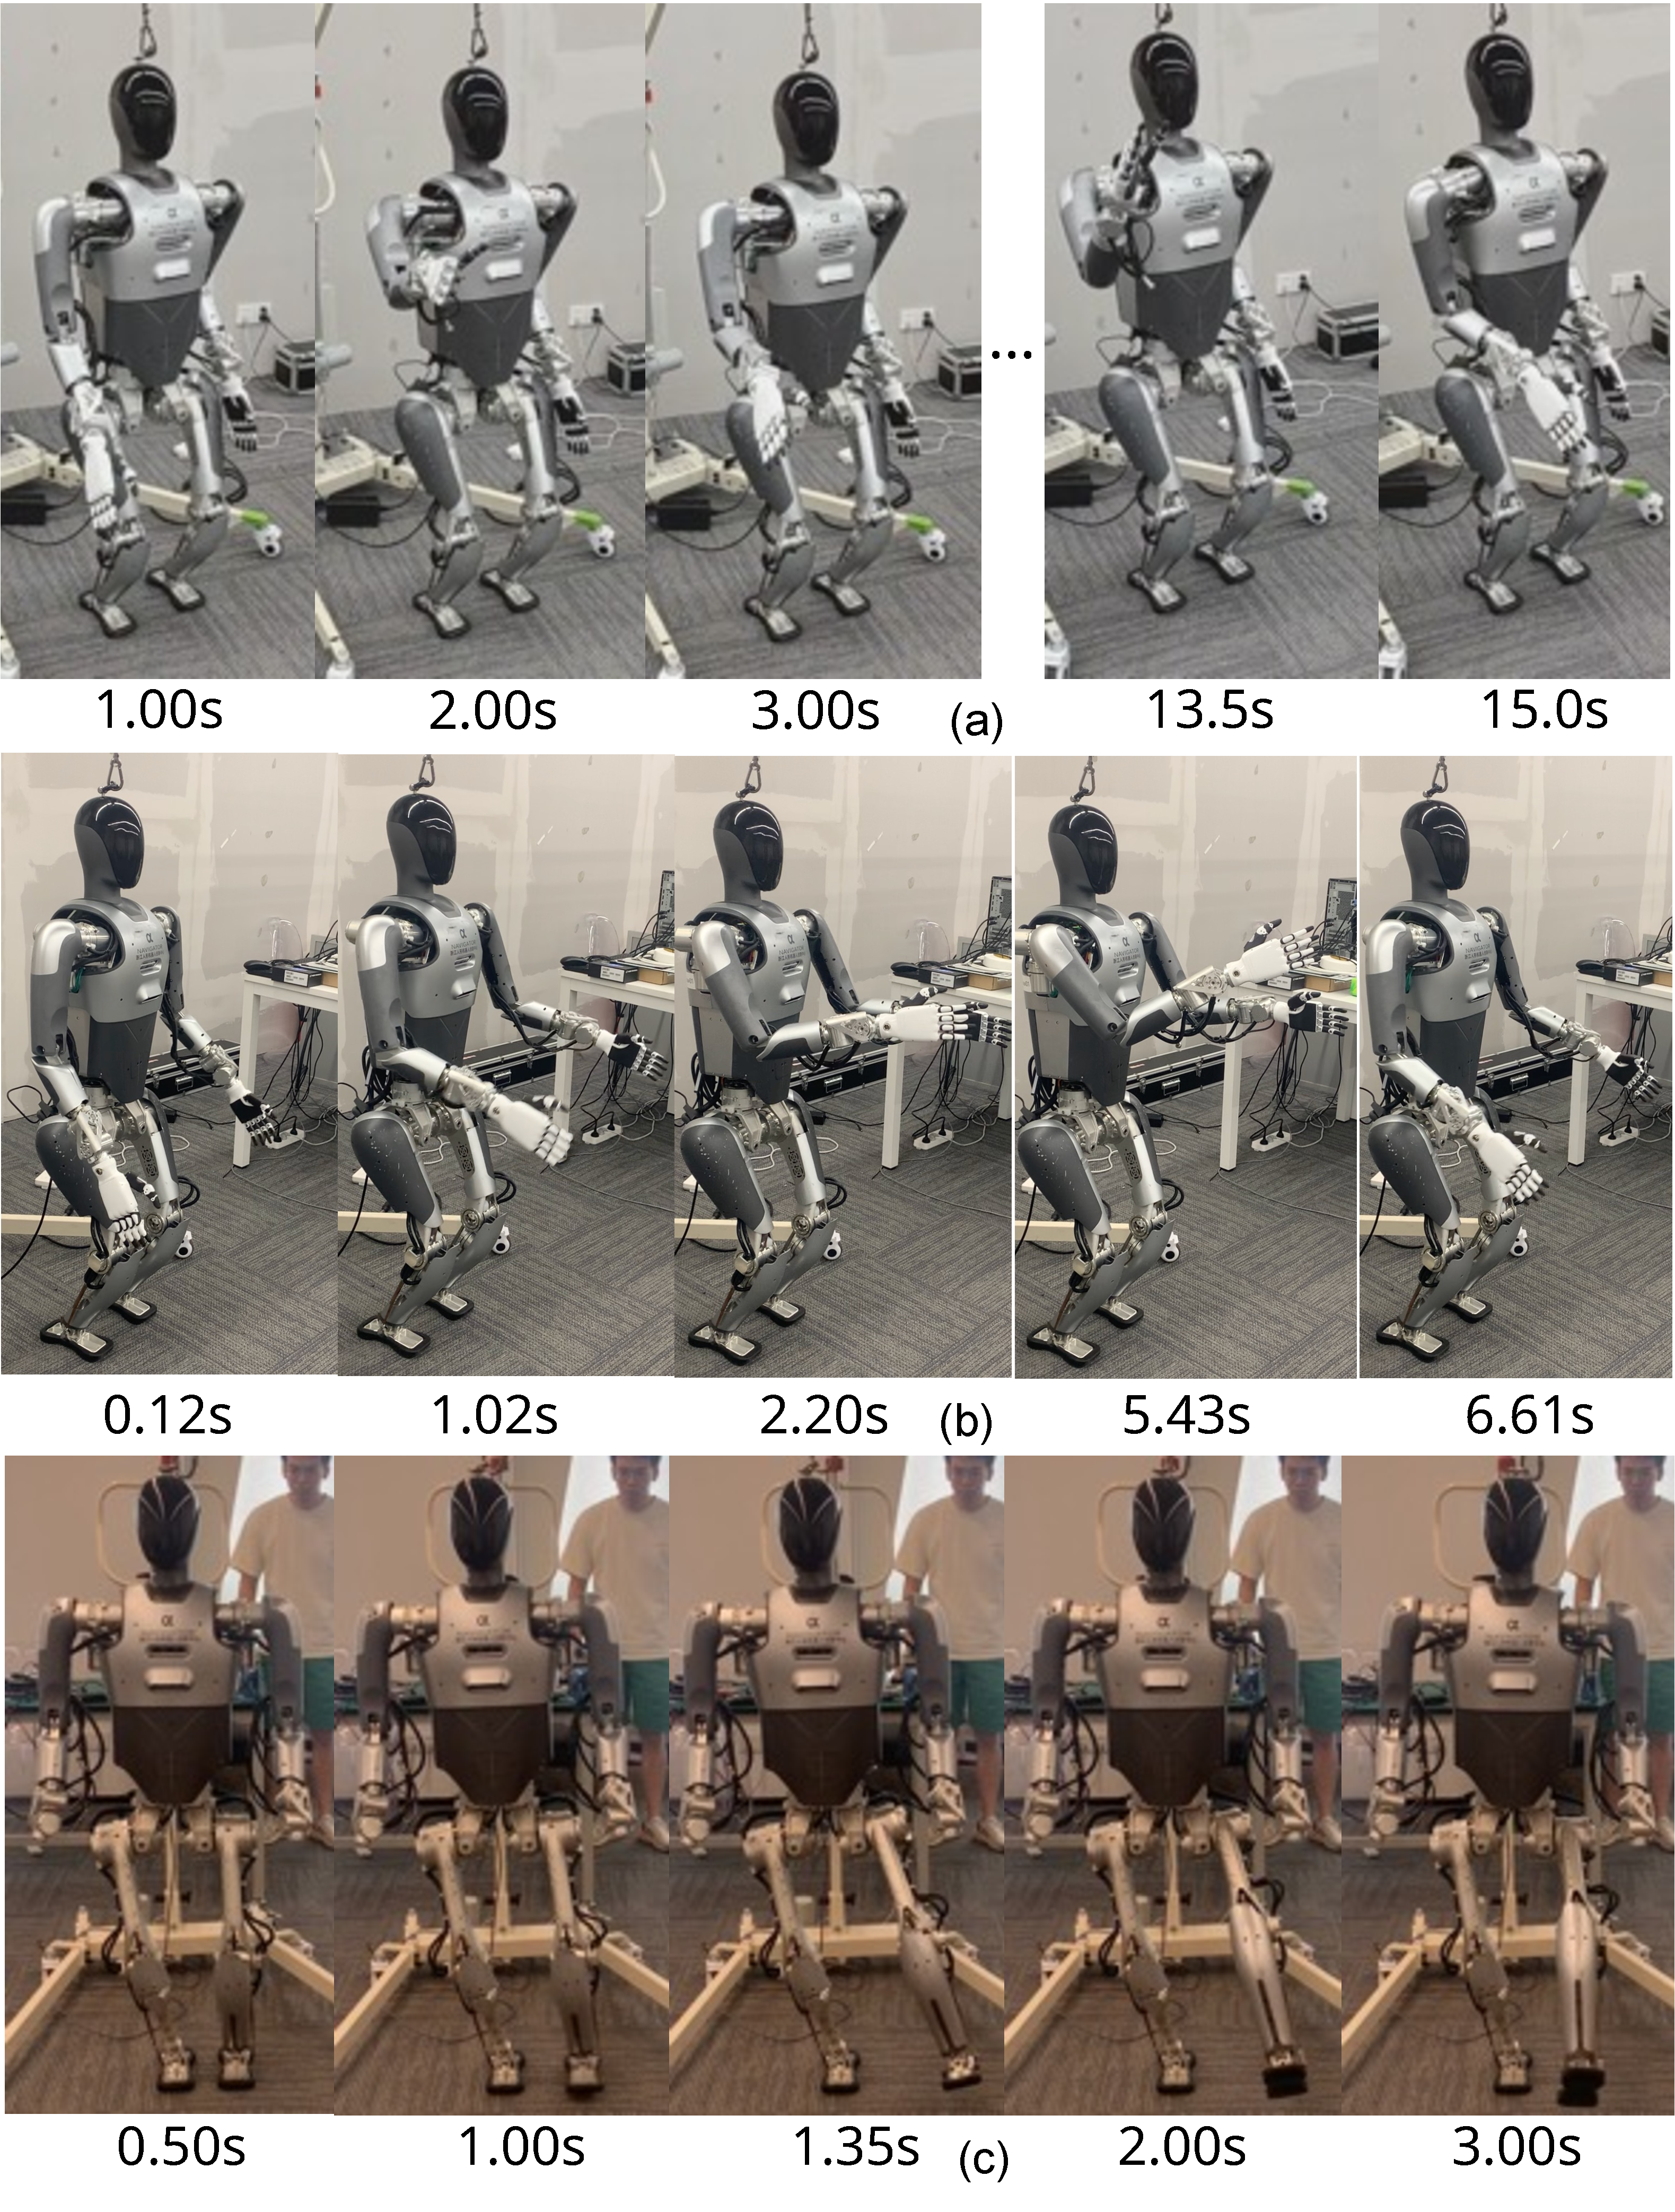
\includegraphics[width=0.4\textwidth]{figures/real_robot.pdf}
      \caption{Screenshots of motion imitation. (a) is the upper-body motion retargeting results both in simulation and real world. (b) shows the motion about hand raising. (c) is the task of standing on one leg. The rope in the screenshots is only for protection and will not exert any force on the robot, more details are in videos \cite{c38}. }
      \label{fig::real_robot}
      \vspace{-15pt}
\end{figure}


\section{CONCLUSIONS}
% add more details about future works, demphi
In this paper, we propose a novel whole-body motion imitation framework that combines motion retargeting and model-based control for a full-size humanoid robot. The whole-body motion retargeting effectively imitates human motion and captures foot contact, while the model-based controller robustly follows the reference trajectory and adapts to external disturbances. The experimental results show that our method is capable of imitating diverse range of human motions with expressiveness and robustness. The limitation of the proposed method is that it only imitates body motion without dexterous hands, and lacks the consideration about multi-contact maneuvers. Future work will consider extending our method to take into account dexterous hands and multi-contact tasks to achieve more versatile motions. 

\addtolength{\textheight}{0.2cm}   % This command serves to balance the column lengths
                                  % on the last page of the document manually. It shortens
                                  % the textheight of the last page by a suitable amount.
                                  % This command does not take effect until the next page
                                  % so it should come on the page before the last. Make
                                  % sure that you do not shorten the textheight too much.

%%%%%%%%%%%%%%%%%%%%%%%%%%%%%%%%%%%%%%%%%%%%%%%%%%%%%%%%%%%%%%%%%%%%%%%%%%%%%%%%



%%%%%%%%%%%%%%%%%%%%%%%%%%%%%%%%%%%%%%%%%%%%%%%%%%%%%%%%%%%%%%%%%%%%%%%%%%%%%%%%



%%%%%%%%%%%%%%%%%%%%%%%%%%%%%%%%%%%%%%%%%%%%%%%%%%%%%%%%%%%%%%%%%%%%%%%%%%%%%%%%


% \section*{ACKNOWLEDGMENT}

% The preferred spelling of the word ÒacknowledgmentÓ in America is without an ÒeÓ after the ÒgÓ. Avoid the stilted expression, ÒOne of us (R. B. G.) thanks . . .Ó  Instead, try ÒR. B. G. thanksÓ. Put sponsor acknowledgments in the unnumbered footnote on the first page.



%%%%%%%%%%%%%%%%%%%%%%%%%%%%%%%%%%%%%%%%%%%%%%%%%%%%%%%%%%%%%%%%%%%%%%%%%%%%%%%%

% References are important to the reader; therefore, each citation must be complete and correct. If at all possible, references should be commonly available publications.



\begin{thebibliography}{99}
\vspace{-5pt}
\bibitem{c1} Dragan, Anca D. et al. "Legibility and predictability of robot motion." \textit{2013 8th ACM/IEEE International Conference on Human-Robot Interaction (HRI). }IEEE, 2013.
\bibitem{c2} Penco, Luigo, et al. "Robust real-time whole-body motion retargeting from human to humanoid." \textit{2018 IEEE-RAS 18th International Conference on Humanoid Robots (Humanoids).} IEEE, 2018.
\bibitem{c3} Elobaid, Mohamed, et al. "Telexistence and teleoperation for walking humanoid robots." \textit{Intelligent Systems and Applications: Proceedings of the 2019 Intelligent Systems Conference (IntelliSys)} Volume 2.
\bibitem{c4} Grandia, Ruben, et al. "Perceptive locomotion through nonlinear model-predictive control." \textit{IEEE Transactions on Robotics 39.5 }(2023): 3402-3421.
\bibitem{c5} Stanton, Christopher, et al. "Teleoperation of a humanoid robot using full-body motion capture, example movements, and machine learning." \textit{Proc. Australasian Conference on Robotics and Automation.} Vol. 8. 2012.
\bibitem{c6} Liarokapis, Minas V., et al. "Directions, methods and metrics for mapping human to robot motion with functional anthropomorphism: A review." \textit{School of Mechanical Engineering, National Technical University of Athens, Tech. Rep} (2013).
\bibitem{c7} Ayusawa, Ko, and Eiichi Yoshida. "Motion retargeting for humanoid robots based on simultaneous morphing parameter identification and motion optimization." \textit{IEEE Transactions on Robotics 33.6 }(2017): 1343-1357.
\bibitem{c8} Miura, Kanako, et al. "Robot motion remix based on motion capture data towards human-like locomotion of humanoid robots." \textit{2009 9th IEEE-RAS International Conference on Humanoid Robots.} IEEE, 2009.
\bibitem{c9} Herr, Hugh, and Marko Popovic. "Angular momentum in human walking." \textit{Journal of experimental biology }211.4 (2008): 467-481.
\bibitem{c10} Zhang, Haodong, et al. "Kinematic motion retargeting via neural latent optimization for learning sign language." \textit{IEEE Robotics and Automation Letters} 7.2 (2022): 4582-4589.
\bibitem{c11} R. Villegas, J. Yang et al., “Neural kinematic networks for unsupervised motion retargetting,” \textit{in IEEE/CVF Conf. on Computer Vision and Pattern Recognition, Jun 2018.}
\bibitem{c12} Peng, Xue Bin, et al. "Amp: Adversarial motion priors for stylized physics-based character control." \textit{ACM Transactions on Graphics (ToG)} 40.4 (2021): 1-20.
\bibitem{c13} Grandia, Ruben, et al. "Doc: Differentiable optimal control for retargeting motions onto legged robots." \textit{ACM Transactions on Graphics (TOG)} 42.4 (2023): 1-14.
\bibitem{c14} Dariush, Behzad, et al. "Online transfer of human motion to humanoids." \textit{International Journal of Humanoid Robotics 6.02} (2009): 265-289.
\bibitem{c15}Ishiguro, Yasuhiro, et al. "Bipedal oriented whole body master-slave system for dynamic secured locomotion with lip safety constraints." \textit{2017 IEEE/RSJ International Conference on Intelligent Robots and Systems (IROS)}. IEEE, 2017.
\bibitem{c16} Otani, et al. "Generating assistive humanoid motions for co-manipulation tasks with a multi-robot quadratic program controller." \textit{2018 IEEE International Conference on Robotics and Automation (ICRA).} IEEE, 2018.
\bibitem{c17} Penco, Luigi, et al. "A multimode teleoperation framework for humanoid loco-manipulation: An application for the icub robot." \textit{IEEE Robotics Automation Magazine 26.4 }(2019): 73-82.
\bibitem{c18} Romualdi, Giulio, et al. "Online non-linear centroidal mpc for humanoid robot locomotion with step adjustment." \textit{2022 International Conference on Robotics and Automation (ICRA)}. IEEE, 2022.
\bibitem{c19} Miura, Kanako, et al. "Robot motion remix based on motion capture data towards human-like locomotion of humanoid robots." \textit{2009 9th IEEE-RAS International Conference on Humanoid Robots. }IEEE, 2009. 
\bibitem{c20} Pollard, Nancy S., et al. "Adapting human motion for the control of a humanoid robot." \textit{Proceedings 2002 IEEE international conference on robotics and automation (Cat. No. 02CH37292)}. Vol. 2. IEEE, 2002.
\bibitem{c21} KDarvish, Kourosh, et al. "Whole-body geometric retargeting for humanoid robots." \textit{2019 IEEE-RAS 19th International Conference on Humanoid Robots (Humanoids). }IEEE, 2019.
\bibitem{c22} Ishiguro, Yasuhiro, et al. "High speed whole body dynamic motion experiment with real time master-slave humanoid robot system." \textit{2018 IEEE International Conference on Robotics and Automation (ICRA).} IEEE, 2018.
\bibitem{c23} Yamane, Katsu, Stuart O. Anderson, and Jessica K. Hodgins. "Controlling humanoid robots with human motion data: Experimental validation." \textit{2010 10th IEEE-RAS International Conference on Humanoid Robots}. IEEE, 2010.
\bibitem{c24} Righetti, Ludovic, et al. "Quadratic programming for inverse dynamics with optimal distribution of contact forces." \textit{2012 12th IEEE-RAS International Conference on Humanoid Robots (Humanoids 2012)}. IEEE, 2012.
\bibitem{c25} Al Borno, Mazen, et al. "Robust Physics‐based Motion Retargeting with Realistic Body Shapes." \textit{Computer Graphics Forum.} Vol. 37. No. 8. 2018.
\bibitem{c26} Hwangbo, Jemin, Joonho Lee, and Marco Hutter. "Per-contact iteration method for solving contact dynamics." \textit{IEEE Robotics and Automation Letters }3.2 (2018): 895-902.
%\bibitem{c27} Carpentier, Justin, et al. "The Pinocchio C++ library: A fast and flexible implementation of rigid body dynamics algorithms and their analytical derivatives." \textit{2019 IEEE/SICE International Symposium on System Integration (SII). }IEEE, 2019.
\bibitem{c28} F. Farshidian et al., “OCS2: An open source library for optimal control of switched systems,” [Online]. Available: https://github.com/leggedrobotics/ocs2.
%\bibitem{c29} H. Ferreau, C. Kirches, A. Potschka, H. Bock, and M. Diehl, “qpOASES: A parametric active-set algorithm for quadratic programming,” \textit{Mathematical Programming Computation}, vol. 6, no. 4, pp. 327–363, 2014.
\bibitem{c30} Mahmood, Naureen, et al. "AMASS: Archive of motion capture as surface shapes." \textit{Proceedings of the IEEE/CVF international conference on computer vision.} 2019.
\bibitem{c31} Sungjoon Choi, Matt Pan, and Joohyung Kim. “Nonparametric Motion Retargeting for Humanoid Robots on Shared Latent Space”. In: \textit{Proceedings of Robotics: Science and Systems (RSS)} (2020).
%\bibitem{c32} Brian Ichter and Marco Pavone. “Robot motion planning in learned latent spaces”. In:\textit{ IEEE Robotics and Automation Letters} 4.3 (2019), pp. 2407–2414.
\bibitem{c33} M. Diehl, H.G. Bock, et al. “Real-time optimization and nonlinear model predictive control of processes governed by differential-algebraic equations,” \textit{Journal of Process Control}, vol. 12, no. 4, pp. 577 – 585, 2002.
\bibitem{c34} P.-B. Wieber, “Holonomy and nonholonomy in the dynamics of articulated motion,” in \textit{Fast motions in biomechanics and robotics.} Springer, 2006, pp. 411–425.
%\bibitem{c35} D. E. Orin, A. Goswami, and S.-H. Lee, “Centroidal dynamics of a humanoid robot,” \textit{Autonomous Robots}, vol. 35, no. 2-3, pp. 161–176, 2013.
\bibitem{c36} S. Caron, Q.-C. Pham, and Y. Nakamura, “Stability of surface contacts for humanoid robots: Closed-form formulae of the contact wrench cone for rectangular support areas,” \textit{2015 International Conference on Robotics and Automation(ICRA)}. IEEE, 2015.
\bibitem{c37} F. Farshidian, M. Neunert, A. W. Winkler, G. Rey, and J. Buchli, “An efficient optimal planning and control framework for quadrupedal locomotion,” in \textit{International Conference on Robotics and Automation (ICRA)}. IEEE, 2017, pp. 93–100.
\bibitem{c38} “Video of the experimental results.” \href{https://youtu.be/4pYzrXH1aUU}{https://youtu.be/4pYzrXH1aUU} \href{https://www.bilibili.com/video/BV1qhKjeEEQu}{https://www.bilibili.com/video/BV1qhKjeEEQu}  
\bibitem{c39} "https://github.com/qiayuanl/legged\_control"
\end{thebibliography}
\enlargethispage{\baselineskip}



\end{document}
